% Options for packages loaded elsewhere
% Options for packages loaded elsewhere
\PassOptionsToPackage{unicode}{hyperref}
\PassOptionsToPackage{hyphens}{url}
\PassOptionsToPackage{dvipsnames,svgnames,x11names}{xcolor}
%
\documentclass[
  english,
  11pt,
  letterpaper,
  DIV=11,
  numbers=noendperiod]{scrartcl}
\usepackage{xcolor}
\usepackage[top=0.92in,bottom=0.92in,inner=1.0in,outer=1.0in]{geometry}
\usepackage{amsmath,amssymb}
\setcounter{secnumdepth}{5}
\usepackage{iftex}
\ifPDFTeX
  \usepackage[T1]{fontenc}
  \usepackage[utf8]{inputenc}
  \usepackage{textcomp} % provide euro and other symbols
\else % if luatex or xetex
  \usepackage{unicode-math} % this also loads fontspec
  \defaultfontfeatures{Scale=MatchLowercase}
  \defaultfontfeatures[\rmfamily]{Ligatures=TeX,Scale=1}
\fi
\usepackage{lmodern}
\ifPDFTeX\else
  % xetex/luatex font selection
\fi
% Use upquote if available, for straight quotes in verbatim environments
\IfFileExists{upquote.sty}{\usepackage{upquote}}{}
\IfFileExists{microtype.sty}{% use microtype if available
  \usepackage[]{microtype}
  \UseMicrotypeSet[protrusion]{basicmath} % disable protrusion for tt fonts
}{}
\makeatletter
\@ifundefined{KOMAClassName}{% if non-KOMA class
  \IfFileExists{parskip.sty}{%
    \usepackage{parskip}
  }{% else
    \setlength{\parindent}{0pt}
    \setlength{\parskip}{6pt plus 2pt minus 1pt}}
}{% if KOMA class
  \KOMAoptions{parskip=half}}
\makeatother
% Make \paragraph and \subparagraph free-standing
\makeatletter
\ifx\paragraph\undefined\else
  \let\oldparagraph\paragraph
  \renewcommand{\paragraph}{
    \@ifstar
      \xxxParagraphStar
      \xxxParagraphNoStar
  }
  \newcommand{\xxxParagraphStar}[1]{\oldparagraph*{#1}\mbox{}}
  \newcommand{\xxxParagraphNoStar}[1]{\oldparagraph{#1}\mbox{}}
\fi
\ifx\subparagraph\undefined\else
  \let\oldsubparagraph\subparagraph
  \renewcommand{\subparagraph}{
    \@ifstar
      \xxxSubParagraphStar
      \xxxSubParagraphNoStar
  }
  \newcommand{\xxxSubParagraphStar}[1]{\oldsubparagraph*{#1}\mbox{}}
  \newcommand{\xxxSubParagraphNoStar}[1]{\oldsubparagraph{#1}\mbox{}}
\fi
\makeatother


\usepackage{longtable,booktabs,array}
\newcounter{none} % for unnumbered tables
\usepackage{calc} % for calculating minipage widths
% Correct order of tables after \paragraph or \subparagraph
\usepackage{etoolbox}
\makeatletter
\patchcmd\longtable{\par}{\if@noskipsec\mbox{}\fi\par}{}{}
\makeatother
% Allow footnotes in longtable head/foot
\IfFileExists{footnotehyper.sty}{\usepackage{footnotehyper}}{\usepackage{footnote}}
\makesavenoteenv{longtable}
\usepackage{graphicx}
\makeatletter
\newsavebox\pandoc@box
\newcommand*\pandocbounded[1]{% scales image to fit in text height/width
  \sbox\pandoc@box{#1}%
  \Gscale@div\@tempa{\textheight}{\dimexpr\ht\pandoc@box+\dp\pandoc@box\relax}%
  \Gscale@div\@tempb{\linewidth}{\wd\pandoc@box}%
  \ifdim\@tempb\p@<\@tempa\p@\let\@tempa\@tempb\fi% select the smaller of both
  \ifdim\@tempa\p@<\p@\scalebox{\@tempa}{\usebox\pandoc@box}%
  \else\usebox{\pandoc@box}%
  \fi%
}
% Set default figure placement to htbp
\def\fps@figure{htbp}
\makeatother


% definitions for citeproc citations
\NewDocumentCommand\citeproctext{}{}
\NewDocumentCommand\citeproc{mm}{%
  \begingroup\def\citeproctext{#2}\cite{#1}\endgroup}
\makeatletter
 % allow citations to break across lines
 \let\@cite@ofmt\@firstofone
 % avoid brackets around text for \cite:
 \def\@biblabel#1{}
 \def\@cite#1#2{{#1\if@tempswa , #2\fi}}
\makeatother
\newlength{\cslhangindent}
\setlength{\cslhangindent}{1.5em}
\newlength{\csllabelwidth}
\setlength{\csllabelwidth}{3em}
\newenvironment{CSLReferences}[2] % #1 hanging-indent, #2 entry-spacing
 {\begin{list}{}{%
  \setlength{\itemindent}{0pt}
  \setlength{\leftmargin}{0pt}
  \setlength{\parsep}{0pt}
  % turn on hanging indent if param 1 is 1
  \ifodd #1
   \setlength{\leftmargin}{\cslhangindent}
   \setlength{\itemindent}{-1\cslhangindent}
  \fi
  % set entry spacing
  \setlength{\itemsep}{#2\baselineskip}}}
 {\end{list}}
\usepackage{calc}
\newcommand{\CSLBlock}[1]{\hfill\break\parbox[t]{\linewidth}{\strut\ignorespaces#1\strut}}
\newcommand{\CSLLeftMargin}[1]{\parbox[t]{\csllabelwidth}{\strut#1\strut}}
\newcommand{\CSLRightInline}[1]{\parbox[t]{\linewidth - \csllabelwidth}{\strut#1\strut}}
\newcommand{\CSLIndent}[1]{\hspace{\cslhangindent}#1}

\ifLuaTeX
\usepackage[bidi=basic,shorthands=off]{babel}
\else
\usepackage[bidi=default,shorthands=off]{babel}
\fi
\ifLuaTeX
  \usepackage{selnolig} % disable illegal ligatures
\fi


\setlength{\emergencystretch}{3em} % prevent overfull lines

\providecommand{\tightlist}{%
  \setlength{\itemsep}{0pt}\setlength{\parskip}{0pt}}



 


\usepackage{microtype}
\usepackage{booktabs}
\usepackage{longtable}
\usepackage{array}
\usepackage{xcolor}
\usepackage{scrlayer-scrpage}
\usepackage{etoolbox}

\definecolor{PhaseNavy}{HTML}{153B55}
\definecolor{PhaseTeal}{HTML}{0F6573}
\definecolor{PhaseRust}{HTML}{A24D2F}

\clearpairofpagestyles
\ihead{\footnotesize\color{PhaseNavy}Hidden Exactness in Bounded-Factor Stochastic Models}
\ohead{\footnotesize\color{PhaseTeal}Kanav Mehta}
\cfoot{\pagemark}
\setheadsepline{0.35pt}[\color{PhaseTeal}]

\addtokomafont{section}{\color{PhaseNavy}}
\addtokomafont{subsection}{\color{PhaseTeal}}
\addtokomafont{subsubsection}{\color{PhaseTeal}}
\setkomafont{pageheadfoot}{\normalfont}

\AtBeginEnvironment{proof}{\small}
\setlength{\emergencystretch}{2em}
\KOMAoption{captions}{tableheading}
\makeatletter
\@ifpackageloaded{tcolorbox}{}{\usepackage[skins,breakable]{tcolorbox}}
\@ifpackageloaded{fontawesome5}{}{\usepackage{fontawesome5}}
\definecolor{quarto-callout-color}{HTML}{909090}
\definecolor{quarto-callout-note-color}{HTML}{0758E5}
\definecolor{quarto-callout-important-color}{HTML}{CC1914}
\definecolor{quarto-callout-warning-color}{HTML}{EB9113}
\definecolor{quarto-callout-tip-color}{HTML}{00A047}
\definecolor{quarto-callout-caution-color}{HTML}{FC5300}
\definecolor{quarto-callout-color-frame}{HTML}{acacac}
\definecolor{quarto-callout-note-color-frame}{HTML}{4582ec}
\definecolor{quarto-callout-important-color-frame}{HTML}{d9534f}
\definecolor{quarto-callout-warning-color-frame}{HTML}{f0ad4e}
\definecolor{quarto-callout-tip-color-frame}{HTML}{02b875}
\definecolor{quarto-callout-caution-color-frame}{HTML}{fd7e14}
\makeatother
\makeatletter
\@ifpackageloaded{caption}{}{\usepackage{caption}}
\AtBeginDocument{%
\ifdefined\contentsname
  \renewcommand*\contentsname{Table of contents}
\else
  \newcommand\contentsname{Table of contents}
\fi
\ifdefined\listfigurename
  \renewcommand*\listfigurename{List of Figures}
\else
  \newcommand\listfigurename{List of Figures}
\fi
\ifdefined\listtablename
  \renewcommand*\listtablename{List of Tables}
\else
  \newcommand\listtablename{List of Tables}
\fi
\ifdefined\figurename
  \renewcommand*\figurename{Figure}
\else
  \newcommand\figurename{Figure}
\fi
\ifdefined\tablename
  \renewcommand*\tablename{Table}
\else
  \newcommand\tablename{Table}
\fi
}
\@ifpackageloaded{float}{}{\usepackage{float}}
\floatstyle{ruled}
\@ifundefined{c@chapter}{\newfloat{codelisting}{h}{lop}}{\newfloat{codelisting}{h}{lop}[chapter]}
\floatname{codelisting}{Listing}
\newcommand*\listoflistings{\listof{codelisting}{List of Listings}}
\usepackage{amsthm}
\theoremstyle{plain}
\newtheorem{theorem}{Theorem}[section]
\theoremstyle{plain}
\newtheorem{corollary}{Corollary}[section]
\theoremstyle{plain}
\newtheorem{lemma}{Lemma}[section]
\theoremstyle{plain}
\newtheorem{proposition}{Proposition}[section]
\theoremstyle{remark}
\AtBeginDocument{\renewcommand*{\proofname}{Proof}}
\newtheorem*{remark}{Remark}
\newtheorem*{solution}{Solution}
\newtheorem{refremark}{Remark}[section]
\newtheorem{refsolution}{Solution}[section]
\makeatother
\makeatletter
\makeatother
\makeatletter
\@ifpackageloaded{caption}{}{\usepackage{caption}}
\@ifpackageloaded{subcaption}{}{\usepackage{subcaption}}
\makeatother
\usepackage{bookmark}
\IfFileExists{xurl.sty}{\usepackage{xurl}}{} % add URL line breaks if available
\urlstyle{same}
% fallback for those not using the hyperref driver hyperxmp:
\makeatletter
\@ifundefined{xmpquote}{\newcommand{\xmpquote}[1]{#1}}{}
\makeatother
\hypersetup{
  pdftitle={Hidden Exactness in Bounded-Factor Stochastic Models},
  pdfauthor={Kanav Mehta},
  pdflang={en},
  pdfkeywords={\xmpquote{stochastic correlation}, \xmpquote{Bachelier
implied volatility}, \xmpquote{Gaussian scale
mixture}, \xmpquote{leverage}, \xmpquote{Feynman--Kac}, \xmpquote{correlation
matrix}, \xmpquote{Brownian motion on a torus}, \xmpquote{Lévy scale
function}},
  colorlinks=true,
  linkcolor={blue},
  filecolor={Maroon},
  citecolor={Blue},
  urlcolor={Blue},
  pdfcreator={LaTeX via pandoc}}


\title{Hidden Exactness in Bounded-Factor Stochastic Models}
\usepackage{etoolbox}
\makeatletter
\providecommand{\subtitle}[1]{% add subtitle to \maketitle
  \apptocmd{\@title}{\par {\large #1 \par}}{}{}
}
\makeatother
\subtitle{Variance-Mixture Smiles, Leverage Closure, and Phase-Gram
Stationarity}
\author{Kanav Mehta}
\date{August 22, 2026}
\begin{document}
\maketitle
\begin{abstract}
Bounded stochastic factors are often introduced by transforming an
unconstrained driver, but tractability is usually assessed one formula
at a time: an exact marginal may survive while first passage, integrated
functionals, leverage, or matrix admissibility does not. This paper
studies the exactness frontier of the bounded coordinate
\(\rho_t=X_t/\sqrt{X_t^2+c^2}\) and of a related Gaussian-angle Gram
process. Three results organize the analysis. First, for every centered
Gaussian scale mixture with random total standard deviation \(S\), the
Bachelier implied standard deviation satisfies \(I(0)=E[S]\) and
\(I''(0)=E[S^{-1}]-E[S]^{-1}\) whenever the inverse moment is finite.
For the affine correlation clock \(V_T=\beta T+\alpha A_T\),
\(A_T=\int_0^T\rho_s\,ds\), this yields an exact at-the-money Jensen
wedge: \(\rho_{\mathrm{imp}}(0)=E[A_T]/T-
\operatorname{Var}(\sqrt{V_T})/(\alpha T)\), and an exact
local-curvature sign split between baskets and spreads. Second, Brownian
leverage between the factor and asset drivers does not destroy
conditional Gaussianity. It produces a path-dependent conditional mean.
An explicit Itô gauge converts that mean into one endpoint and one
additive functional, while Fourier transformation reduces the terminal
characteristic function of a linear asset combination to a
one-dimensional complex Feynman--Kac equation; European claims with a
valid Fourier representation inherit that closure. Leverage generically
creates skewness, while the standard terminal scalar- clock reflection
derivation for barriers requires additional structure. Third,
independent Brownian triangular angles induce a correlation-matrix
process whose unwrapped coordinates diffuse while its matrix marginals
converge to a compact stationary pushforward law. The determinant has
exact finite-time moments, a stationary
product-\(\operatorname{Beta}(1/2,1/2)\) law, explicit log-cumulants and
a high-dimensional central limit theorem; the survival function of its
first singularity time factors into a product of killed-Brownian
survival probabilities. Supporting sections correct the
scale-identifiability orbit and a nonautonomous Feynman--Kac
operator-ordering error, and record exact endpoint--clock and spectrally
one-sided Lévy extensions. The paper separates these model-specific
results from the classical mixture, evolution-family, hyperspherical,
hypoelliptic, and fluctuation-theory ingredients on which they rest.
\end{abstract}

\renewcommand*\contentsname{Table of contents}
{
\setcounter{tocdepth}{2}
\tableofcontents
}

\textbf{Mathematics Subject Classification (2020):} 60H10, 60J60, 60J65,
60G51, 91G20, 91G60.

\textbf{JEL classification:} C02, C63, G12, G13.

\section{Introduction}\label{sec-introduction}

Correlation is simultaneously a bounded state variable, a latent risk
factor, and an input to every multi-asset variance calculation. Its
stochastic modeling literature contains transform models, Jacobi-type
diffusions, Wishart covariance processes, copula dynamics, and
local-correlation constructions. These approaches solve different pieces
of the same problem: admissibility, mean reversion, finite-time laws,
calibration, or derivative pricing (Skintzi and Refenes 2005; Driessen
et al. 2009; Fonseca et al. 2007; Ma 2009; Gouriéroux and Sufana 2010;
Linders and Schoutens 2014). None of those properties implies the
others.

The distinction matters most for path-dependent claims. A bounded
transform of a Gaussian driver has an immediate marginal law, but a
marginal law does not price an occupation clock, a first-passage claim,
or a barrier on a spread. Conversely, a matrix process can remain
positive semidefinite by construction while its determinant, boundary
behavior, and long-horizon law remain opaque. Exactness is therefore not
binary. It is a ledger of which objects survive a modeling operation.

The bounded coordinate studied here is

\begin{equation}\protect\phantomsection\label{eq-bounded-map}{
\rho_t=f_c(X_t)
=\frac{X_t}{\sqrt{X_t^2+c^2}},
\qquad
c>0.
}\end{equation}

For a Gaussian driver, the map transports transitions and scalar
barriers from the real line to \((-1,1)\). Earlier phases of this
research program used that fact to obtain exact correlation transitions,
reflection-principle barriers, occupation-clock transforms, and
spread/basket prices. The same program introduced a matrix extension:
independent Gaussian triangular angles are inserted into a
hyperspherical Gram factor, guaranteeing a valid correlation matrix at
every time.

The present paper began by auditing where that program claimed exactness
was lost. Several boundaries were drawn too broadly. Independence of the
factor and asset drivers is not necessary for conditional Gaussianity.
Unwrapped Gaussian angles have no invariant probability law on
\(\mathbb R^d\), but the matrix sees only periodic functions of those
angles. The standard two-time backward Feynman--Kac theorem does not
cease to hold when coefficients depend on calendar time; a
time-homogeneous operator ordering ceases to hold. Reflection fails for
generic jump processes, but one-sided Lévy fluctuation identities do
not.

The audit also found two concrete errors worth correcting. First, the
positive scale orbit of the bounded Gaussian model scales
\((x_0,c,\mu,\sigma)\) in the same direction; inverse scaling does not
preserve the normalized process. Second, the at-the-money implied
correlation of a nondegenerate variance mixture is not the mean
correlation clock. The ATM Bachelier price depends on \(E[\sqrt{V_T}]\),
not \(\sqrt{E[V_T]}\).

\subsection{Contributions and claim
taxonomy}\label{contributions-and-claim-taxonomy}

The paper has three principal theorem families and four supporting
corrections or exact extensions; Figure~\ref{fig-contribution} displays
the dependency map.

\begin{figure}[tbp]

\centering{

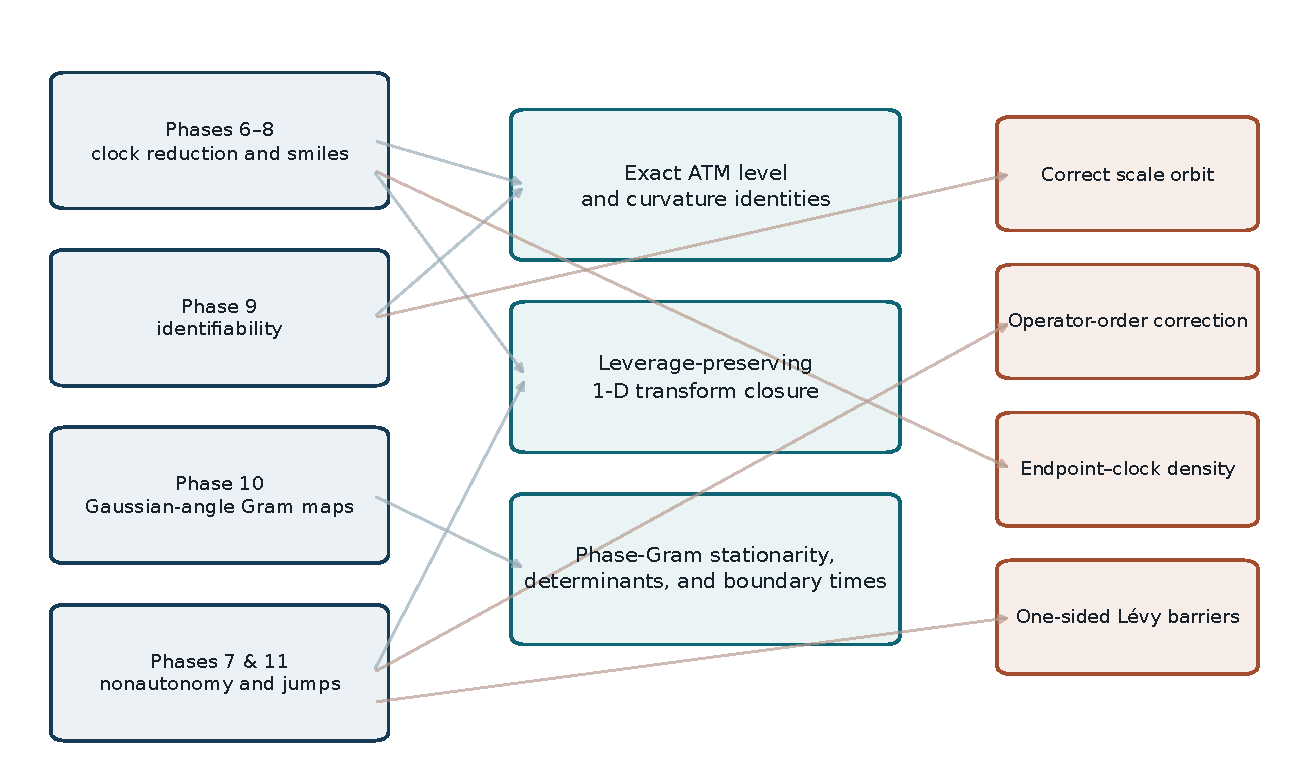
\includegraphics[width=1\linewidth,height=\textheight,keepaspectratio,alt={Flow diagram connecting earlier bounded-factor results to exact ATM smile identities, leverage closure, Phase-Gram stationarity, and four corrected mathematical frontiers.}]{figures/vector/f01_contribution_map.pdf}

}

\caption{\label{fig-contribution}The Phase 14 contribution map. Earlier
clock, identifiability, Gram, nonautonomous, and jump results feed three
main theorem families and four corrected frontiers.}

\end{figure}%

\begin{enumerate}
\def\labelenumi{\arabic{enumi}.}
\tightlist
\item
  \textbf{Clock-specific smile geometry.} For a centered Gaussian scale
  mixture, we derive the exact ATM implied-standard-deviation level and
  curvature. These are compact specializations of established Bachelier
  stochastic- volatility calculations (Renault and Touzi 1996; Alòs et
  al. 2024; Alòs and García-Lorite 2025; Alòs and Burés Mogollón 2026).
  Their use here is the exact correlation-clock corollary: the ATM
  Jensen wedge and opposite local basket/spread curvature signs.
\item
  \textbf{Bounded-factor leverage closure.} We derive the admissible
  Brownian leverage geometry, the conditional random-mean Gaussian law,
  an explicit endpoint--additive Itô gauge, a one-dimensional transform
  PDE, and a short-time third-moment coefficient. Conditional mixing and
  Fourier reduction under leverage are established ideas (Willard 1997;
  Alòs 2006; Heston 1993; Das and Langrené 2022); the contribution is
  their exact specialization and frontier in the bounded-factor system.
\item
  \textbf{Dynamic Phase-Gram analysis.} The hyperspherical map and
  determinant factorization are classical (Pinheiro and Bates 1996;
  Rebonato and Jäckel 2000; Rapisarda et al. 2007; Pourahmadi and Wang
  2015; Forrester and Zhang 2020). We derive the finite-time determinant
  moments, compact stationary pushforward, product-Beta equilibrium
  determinant, and first matrix-singularity law for the specified
  Brownian-angle dynamics.
\item
  \textbf{Corrections and exact extensions.} We repair the scale orbit
  and nonautonomous operator ordering, derive the smooth joint
  endpoint--clock density through a tilted one-dimensional kernel, and
  transfer classical one-sided Lévy scale-function barriers through the
  bounded map.
\end{enumerate}

\begin{tcolorbox}[enhanced jigsaw, arc=.35mm, bottomrule=.15mm, breakable, colback=white, colframe=quarto-callout-note-color-frame, left=2mm, leftrule=.75mm, opacityback=0, rightrule=.15mm, toprule=.15mm]
\begin{minipage}[t]{5.5mm}
\textcolor{quarto-callout-note-color}{\faInfo}
\end{minipage}%
\begin{minipage}[t]{\textwidth - 5.5mm}

\vspace{-3mm}\textbf{Claim categories used throughout}\vspace{3mm}

\textbf{Project-specific result} means a theorem or calculation derived
for the particular bounded-factor or Brownian-angle model.
\textbf{Correction} means a previous statement in this research program
was mathematically inaccurate or too broad. \textbf{Classical
specialization} means the theorem follows by applying established
machinery to this coordinate. No category by itself is a claim of world
priority.

\end{minipage}%
\end{tcolorbox}

\subsection{Related work and the novelty
boundary}\label{related-work-and-the-novelty-boundary}

The normal option formula originates with Bachelier (Bachelier 1900).
Modern treatments address stable inversion and the relation between
normal and lognormal quotation (Choi et al. 2009, 2022; Jäckel 2017).
Arithmetic-Brownian spread pricing and the broader spread-option problem
are treated by Poitras (1998) and Carmona and Durrleman (2003).

Normal scale and variance-mean mixtures are classical probability
objects (Andrews and Mallows 1974; Barndorff-Nielsen et al. 1982), and
stochastic clocks have a long financial history (Clark 1973). In the
independent stochastic-volatility setting, the terminal law is an
integrated-variance mixture (Hull and White 1987), with symmetric
implied-smile consequences (Renault and Touzi 1996). Recent Bachelier
work obtains ATM levels, skews, curvatures, and moneyness expansions
under broad, sometimes rough, stochastic-volatility assumptions (Alòs et
al. 2024; Alòs and García-Lorite 2025; Alòs and Burés Mogollón 2026).
Section Section~\ref{sec-smiles} therefore does not claim the general
subject of Bachelier curvature. Its distinctive object is the affine
correlation clock and the exact conversion of clock dispersion into
opposite implied-correlation corrections.

Stochastic correlation is a mature multi-asset modeling problem.
Empirical and model-dependent implied-correlation measures are developed
by Skintzi and Refenes (2005), Driessen et al. (2009), and Linders and
Schoutens (2014). Stochastic-covariance and direct stochastic-
correlation models provide analytical or numerical multi-asset pricing
(Fonseca et al. 2007; Ma 2009; Escobar et al. 2009, 2016; Gouriéroux and
Sufana 2010). The paper does not infer novelty from boundedness alone.

Likewise, leverage need not destroy transform or conditional-mixing
methods. Correlated stochastic-volatility models, affine transforms, and
random-mean mixing formulas already demonstrate that fact (Romano and
Touzi 1997; Willard 1997; Alòs 2006; Heston 1993; Scott 1997; Duffie et
al. 2000; Das and Langrené 2022). Barrier reductions may also survive
under structures different from the one considered here (Rolloos 2022).
Section Section~\ref{sec-leverage} consequently makes a narrower claim:
the earlier assertion that leverage destroys conditional Gaussianity in
this bounded-factor model is false, and its correct replacement is an
explicit random-mean law and one-dimensional complex Feynman--Kac
transform.

The matrix section sits beside a substantial literature on unconstrained
covariance parameterizations, random correlation matrices, and
determinant-power laws (Joe 2006; Lewandowski et al. 2009; Muirhead
1982; Holmes 1991; Bendel and Mickey 1978; Barnard et al. 2000; Archakov
et al. 2024). Dynamic hyperspherical parameters are themselves not new
(Buccheri et al. 2021). The flat-angle invariant law derived below is
neither uniform on the elliptope nor LKJ. That distinction is essential.

\subsection{Organization}\label{organization}

Section Section~\ref{sec-framework} fixes the model and notation.
Section Section~\ref{sec-smiles} develops the exact centered-mixture
identities and their correlation-clock consequences. Section
Section~\ref{sec-leverage} treats Brownian leverage. Section
Section~\ref{sec-phasegram} derives the matrix laws. Section
Section~\ref{sec-frontiers} contains the four supporting corrections and
exact extensions. Section Section~\ref{sec-implications} assembles the
tractability map, limitations, and open problems. Appendices collect
calculations that would interrupt the main argument.

\section{Bounded-factor framework and conventions}\label{sec-framework}

\subsection{Probability space and scalar
factor}\label{probability-space-and-scalar-factor}

Work on a filtered probability space
\((\Omega,\mathcal F,(\mathcal F_t)_{t\ge0},\mathbb P)\) satisfying the
usual conditions. Unless another measure is stated, every Brownian
motion is standard under \(\mathbb P\). Fix

\begin{equation}\protect\phantomsection\label{eq-fs}{
c>0,\qquad
f_c(x)=\frac{x}{\sqrt{x^2+c^2}},
\qquad
s_c(x)=\frac{c}{\sqrt{x^2+c^2}}.
}\end{equation}

Then \(f_c^2+s_c^2=1\), \(f_c\) is a smooth increasing homeomorphism
from \(\mathbb R\) to \((-1,1)\), and

\begin{equation}\protect\phantomsection\label{eq-inverse}{
f_c^{-1}(r)=\frac{cr}{\sqrt{1-r^2}},
\qquad
\frac{d}{dr}f_c^{-1}(r)=\frac{c}{(1-r^2)^{3/2}}.
}\end{equation}

The baseline Gaussian factor is

\begin{equation}\protect\phantomsection\label{eq-factor}{
dX_t=\mu\,dt+\nu\,dW_t^0,\qquad
X_0=x_0,\qquad \nu>0,
}\end{equation}

and the bounded state is \(\rho_t=f_c(X_t)\). On every finite interval
the state remains strictly inside \((-1,1)\).

\subsection{Two forwards and a linear
combination}\label{two-forwards-and-a-linear-combination}

Let \(W^1,W^2\) be Brownian motions with \(d[W^1,W^2]_t=0\). Under the
independence specification used in Section Section~\ref{sec-smiles},
\(W^0\) is independent of \((W^1,W^2)\). The two Bachelier forward
prices satisfy

\[
dF_{1,t}=\sigma_1\,dW_t^1,
\]

\begin{equation}\protect\phantomsection\label{eq-two-forwards}{
dF_{2,t}=\sigma_2
\left(
\rho_t\,dW_t^1+s_c(X_t)\,dW_t^2
\right).
}\end{equation}

Thus

\[
d[F_1,F_2]_t=\sigma_1\sigma_2\rho_t\,dt.
\]

For constants \(\alpha_1,\alpha_2\), define

\begin{equation}\protect\phantomsection\label{eq-linear-combination}{
Z_t=\alpha_1F_{1,t}+\alpha_2F_{2,t},
\qquad
p=\alpha_1\sigma_1,\qquad
q=\alpha_2\sigma_2.
}\end{equation}

The instantaneous variance rate is

\begin{equation}\protect\phantomsection\label{eq-Q}{
Q(x)
=(p+qf_c(x))^2+q^2s_c(x)^2
=p^2+q^2+2pqf_c(x).
}\end{equation}

Write

\begin{equation}\protect\phantomsection\label{eq-clock-definitions}{
\beta=p^2+q^2,\qquad
\alpha=2pq,\qquad
A_T=\int_0^T\rho_t\,dt.
}\end{equation}

Under independence,

\begin{equation}\protect\phantomsection\label{eq-centered-clock-law}{
Z_T\mid\rho_{[0,T]}
\sim N(z_0,V_T),
\qquad
V_T=\beta T+\alpha A_T.
}\end{equation}

Since \(|A_T|<T\), the total variance lies between \((\beta-|\alpha|)T\)
and \((\beta+|\alpha|)T\). We assume it is strictly positive in every
result requiring an inverse square-root moment.

\subsection{Conventions under
leverage}\label{conventions-under-leverage}

Section Section~\ref{sec-leverage} permits

\begin{equation}\protect\phantomsection\label{eq-leverage-brackets}{
d[W^0,W^1]_t=\ell_1\,dt,\qquad
d[W^0,W^2]_t=\ell_2\,dt,
\qquad
d[W^1,W^2]_t=0.
}\end{equation}

Whenever a covariance matrix is displayed, the coordinate order is
stated. The symbols \(q\) and \(\delta\) are deliberately separated:
\(q\) is the signed asset loading in Eq.~\ref{eq-linear-combination},
whereas \(\delta\ge0\) is the killing or discount rate in Lévy
fluctuation identities.

An equality conditional on \(X\) is an equality of regular conditional
laws. When a clock \(J\) is strictly increasing, the notation
\(J^{-1}(v)=\inf\{t:J_t\ge v\}\) denotes its time inverse. No
inverse-clock representation is imposed when \(J\) has flat intervals.

\subsection{Phase-Gram construction}\label{phase-gram-construction}

For \(n\) assets let \(d=n(n-1)/2\). For \(i>j\), let \(\theta_{ij}\) be
a triangular angle. Define the lower-triangular hyperspherical Gram
factor \(B(\theta)\) by

\[
B_{i,k}
=\cos\theta_{ik}\prod_{m<k}\sin\theta_{im},
\qquad k<i,
\]

\begin{equation}\protect\phantomsection\label{eq-gram-factor}{
B_{i,i}=\prod_{m<i}\sin\theta_{im},
\qquad B_{1,1}=1,
}\end{equation}

and set

\begin{equation}\protect\phantomsection\label{eq-gram-map}{
R(\theta)=B(\theta)B(\theta)^\top.
}\end{equation}

Every row of \(B\) has unit Euclidean norm, so \(R\) is symmetric
positive semidefinite with unit diagonal. Outside the canonical chart
\(0<\theta_{ij}<\pi\), diagonal entries of \(B\) can be negative; ``Gram
factor'' is therefore more accurate than ``Cholesky factor.''

The dynamic model is

\begin{equation}\protect\phantomsection\label{eq-angle-bm}{
d\theta_j(t)=\sigma_j\,dW_j(t),
\qquad \sigma_j>0,
\qquad j=1,\ldots,d,
}\end{equation}

with independent drivers. Initial angles are deterministic for
finite-time product formulas unless stated otherwise. A stationary
random initialization is independent of future Brownian increments.

\subsection{Notation and hypothesis
ledger}\label{notation-and-hypothesis-ledger}

\begin{longtable}[]{@{}
  >{\raggedright\arraybackslash}p{(\linewidth - 2\tabcolsep) * \real{0.5000}}
  >{\raggedright\arraybackslash}p{(\linewidth - 2\tabcolsep) * \real{0.5000}}@{}}
\caption{Standing notation and
qualifications.}\label{tbl-notation}\tabularnewline
\toprule\noalign{}
\begin{minipage}[b]{\linewidth}\raggedright
Symbol or phrase
\end{minipage} & \begin{minipage}[b]{\linewidth}\raggedright
Meaning and standing condition
\end{minipage} \\
\midrule\noalign{}
\endfirsthead
\toprule\noalign{}
\begin{minipage}[b]{\linewidth}\raggedright
Symbol or phrase
\end{minipage} & \begin{minipage}[b]{\linewidth}\raggedright
Meaning and standing condition
\end{minipage} \\
\midrule\noalign{}
\endhead
\bottomrule\noalign{}
\endlastfoot
\(f_c,s_c\) & Bounded coordinate and positive complement in
Eq.~\ref{eq-fs}, with \(c>0\). \\
\(S=\sqrt V\) & Random total standard deviation; \(S>0\) almost
surely. \\
\(I(k)\) & Bachelier total implied standard deviation at signed
moneyness \(k=K-z_0\). \\
\(\rho_{\mathrm{imp}}(k)\) & Constant correlation matching the mixture
call, when the inversion lies in \([-1,1]\). \\
\(\ell=(\ell_1,\ell_2)\) & Primitive Brownian leverage vector;
\(\|\ell\|^2\le1\). \\
\(\Gamma\) & Residual conditional variance rate under leverage. \\
\(\Pi_n\) & Pushforward of product-uniform angle measure through the
Gram map. \\
\(Q_{s,t}\) & Two-time tilted evolution family; generator domains share
an invariant core when commutators are used. \\
\(K_\xi\) & Fourier-tilted endpoint kernel, with inversion
distributional unless \(L^1_\xi\) decay is proved. \\
\(W^{(\delta)},Z^{(\delta)}\) & Spectrally negative Lévy scale functions
under the normalization in Section Section~\ref{sec-levy}. \\
\end{longtable}

\subsection{Reproducible numerical
role}\label{reproducible-numerical-role}

All figures and numerical tables are generated by one deterministic
script with seed 20260822. The numerical layer checks the exact
identities against independent quadrature or simulation. It is not used
to infer a theorem. The reference clock parameters are

\begin{equation}\protect\phantomsection\label{eq-reference-parameters}{
\sigma_1=1.5,\quad
\sigma_2=2.5,\quad
x_0=0,\quad
\mu=0.3,\quad
\nu=0.8,\quad
c=T=1.
}\end{equation}

\section{Exact variance-mixture smile geometry}\label{sec-smiles}

\subsection{Centered Gaussian scale
mixtures}\label{centered-gaussian-scale-mixtures}

Let \(S>0\) be a random variable and suppose that, conditional on \(S\),

\begin{equation}\protect\phantomsection\label{eq-scale-mixture}{
Y\mid S\sim N(0,S^2).
}\end{equation}

This is the centered normal scale-mixture structure studied classically
in probability (Andrews and Mallows 1974; Barndorff-Nielsen et al.
1982). In the independent-clock model Eq.~\ref{eq-centered-clock-law},
\(Y=Z_T-z_0\) and \(S=\sqrt{V_T}\). Conditional normality depends only
on the clock; the detailed path producing that clock is irrelevant for a
terminal European payoff.

For signed moneyness

\[
k=K-z_0,
\]

the undiscounted centered Bachelier call is

\begin{equation}\protect\phantomsection\label{eq-bachelier-call}{
\mathcal B(s,k)
=s\varphi(k/s)-k\Phi(-k/s),
\qquad s>0,
}\end{equation}

where \(\varphi\) and \(\Phi\) are the standard normal density and
distribution function. The mixture call is

\begin{equation}\protect\phantomsection\label{eq-mixture-call}{
C(k)=E[\mathcal B(S,k)].
}\end{equation}

The total implied standard deviation \(I(k)\) is defined by

\begin{equation}\protect\phantomsection\label{eq-implied-definition}{
\mathcal B(I(k),k)=C(k).
}\end{equation}

This convention quotes total standard deviation, not annualized normal
volatility. The two differ by \(\sqrt T\).

\begin{lemma}[Bachelier derivatives and
inversion]\protect\hypertarget{lem-bachelier-calculus}{}\label{lem-bachelier-calculus}

For \(s>0\),

\[
\mathcal B_s(s,k)=\varphi(k/s)>0,
\]

\[
\mathcal B_k(s,k)=-\Phi(-k/s),
\qquad
\mathcal B_{kk}(s,k)=\frac{\varphi(k/s)}{s}.
\]

If \(E[S]<\infty\), then for every \(k\) the mixture price lies strictly
above intrinsic value and Eq.~\ref{eq-implied-definition} has a unique
solution \(I(k)>0\).

\end{lemma}

\begin{proof}
Differentiate Eq.~\ref{eq-bachelier-call} directly, using
\(\varphi'(x)=-x\varphi(x)\). The terms produced by differentiating
\(s\varphi(k/s)\) and \(-k\Phi(-k/s)\) cancel in the first derivatives.
Strict positivity of \(\mathcal B_s\) gives strict monotonicity in
\(s\).

For fixed \(k\), \(\mathcal B(s,k)\) increases continuously from
\((-k)^+\) as \(s\downarrow0\) to infinity as \(s\uparrow\infty\).
Because \(S>0\) almost surely, \(\mathcal B(S,k)>(-k)^+\) almost surely,
hence \(C(k)>(-k)^+\). Integrability follows from the elementary bound
\(\mathcal B(S,k)\le S/\sqrt{2\pi}+(-k)^+\). The intermediate-value
theorem and strict monotonicity complete the proof. \(\square\)
\end{proof}

Normal implied-volatility inversion has its own numerical literature
(Choi et al. 2009, 2022; Jäckel 2017). Here inversion is used
analytically; no approximation formula is required.

\subsection{Exact level and curvature}\label{exact-level-and-curvature}

\begin{theorem}[Exact centered-mixture ATM
identities]\protect\hypertarget{thm-mixture-smile}{}\label{thm-mixture-smile}

Assume

\[
0<E[S]<\infty.
\]

Then the total implied standard deviation is even and

\begin{equation}\protect\phantomsection\label{eq-mixture-level}{
\boxed{
I(-k)=I(k),\qquad I(0)=E[S].
}
}\end{equation}

If additionally

\begin{equation}\protect\phantomsection\label{eq-inverse-moment}{
E[S^{-1}]<\infty,
}\end{equation}

then \(I\) is twice differentiable at zero and

\begin{equation}\protect\phantomsection\label{eq-mixture-curvature}{
\boxed{
I''(0)=E[S^{-1}]-\frac1{E[S]}.
}
}\end{equation}

Consequently,

\begin{equation}\protect\phantomsection\label{eq-implied-variance-curvature}{
\boxed{
(I^2)''(0)
=2\left(E[S]E[S^{-1}]-1\right)\ge0.
}
}\end{equation}

Equality in Eq.~\ref{eq-implied-variance-curvature} holds if and only if
\(S\) is constant almost surely.

\end{theorem}

\begin{proof}
The Bachelier parity identity in signed-moneyness form is

\begin{equation}\protect\phantomsection\label{eq-bachelier-parity}{
\mathcal B(s,-k)=\mathcal B(s,k)+k.
}\end{equation}

Taking expectations in Eq.~\ref{eq-mixture-call},

\[
C(-k)=C(k)+k.
\]

If \(I(k)\) solves Eq.~\ref{eq-implied-definition}, then

\[
\mathcal B(I(k),-k)
=\mathcal B(I(k),k)+k
=C(-k).
\]

Uniqueness from Lemma~\ref{lem-bachelier-calculus} implies
\(I(-k)=I(k)\).

At zero moneyness,

\[
\mathcal B(s,0)=\varphi(0)s.
\]

Therefore

\[
\varphi(0)I(0)
=C(0)
=\varphi(0)E[S],
\]

which proves the level.

For curvature, Lemma~\ref{lem-bachelier-calculus} gives

\[
C'(0)=-\frac12.
\]

Under Eq.~\ref{eq-inverse-moment}, differentiation under the expectation
is justified near zero by

\[
0\le
\frac{\varphi(k/S)}{S}
\le
\frac{\varphi(0)}{S},
\]

so

\begin{equation}\protect\phantomsection\label{eq-mixture-price-second}{
C''(0)=\varphi(0)E[S^{-1}].
}\end{equation}

Differentiate Eq.~\ref{eq-implied-definition} once:

\[
\mathcal B_s(I(k),k)I'(k)
+\mathcal B_k(I(k),k)
=C'(k).
\]

At \(k=0\), both \(\mathcal B_k\) and \(C'\) equal \(-1/2\), while
\(\mathcal B_s=\varphi(0)\), hence \(I'(0)=0\). A second differentiation
gives

\[
\mathcal B_s I''
+\mathcal B_{ss}(I')^2
+2\mathcal B_{sk}I'
+\mathcal B_{kk}
=C''.
\]

At zero,

\[
\mathcal B_{ss}=\mathcal B_{sk}=I'=0,
\qquad
\mathcal B_s=\varphi(0),
\qquad
\mathcal B_{kk}=\frac{\varphi(0)}{I(0)}.
\]

Combine these identities with Eq.~\ref{eq-mixture-price-second} and
\(I(0)=E[S]\) to obtain Eq.~\ref{eq-mixture-curvature}.

Finally,

\[
(I^2)''(0)=2I(0)I''(0)
=2(E[S]E[S^{-1}]-1).
\]

Cauchy--Schwarz applied to \(\sqrt S\) and \(1/\sqrt S\) gives
\(E[S]E[S^{-1}]\ge1\). Equality requires \(\sqrt S\) and \(1/\sqrt S\)
to be linearly dependent almost surely, hence \(S\) is constant.
\(\square\)
\end{proof}

\begin{tcolorbox}[enhanced jigsaw, arc=.35mm, bottomrule=.15mm, breakable, colback=white, colframe=quarto-callout-important-color-frame, left=2mm, leftrule=.75mm, opacityback=0, rightrule=.15mm, toprule=.15mm]
\begin{minipage}[t]{5.5mm}
\textcolor{quarto-callout-important-color}{\faExclamation}
\end{minipage}%
\begin{minipage}[t]{\textwidth - 5.5mm}

\vspace{-3mm}\textbf{Literature boundary}\vspace{3mm}

Theorem Theorem~\ref{thm-mixture-smile} is an exact finite-horizon
specialization of a well-developed Bachelier stochastic-volatility
literature. Alòs et al. (2024) treats ATM level, skew, and short-time
behavior; Alòs and García-Lorite (2025) gives the exact fixed-maturity
Bachelier curvature decomposition; and Alòs and Burés Mogollón (2026)
supplies a negative-half-moment moneyness expansion. The compact
inverse-moment form is useful here because it exposes the
correlation-clock sign algebra immediately; it is not presented as the
invention of Bachelier curvature.

\end{minipage}%
\end{tcolorbox}

The inverse-moment condition is substantive. If \(S\) approaches zero
too quickly, \(C''(0)\) and \(I''(0)\) can be infinite. For example, a
scale uniformly distributed on \((0,1)\) has finite mean but infinite
\(E[S^{-1}]\).

\subsection{Correlation inversion and the ATM Jensen
wedge}\label{correlation-inversion-and-the-atm-jensen-wedge}

Return to

\[
S^2=V_T=\beta T+\alpha A_T,
\qquad \alpha\ne0.
\]

The constant-correlation Bachelier comparator has total variance

\[
V_T^{\mathrm{const}}(\rho)=\beta T+\alpha T\rho.
\]

Define the implied correlation by

\begin{equation}\protect\phantomsection\label{eq-implied-correlation}{
I(k)^2=\beta T+\alpha T\rho_{\mathrm{imp}}(k).
}\end{equation}

Because \(A_T/T\in(-1,1)\), the random total standard deviation lies
between the two constant-correlation endpoint values. Monotonicity of
the Bachelier call in \(s\) implies that \(I(k)\) lies in the same
interval; therefore \(\rho_{\mathrm{imp}}(k)\in[-1,1]\) whenever the
endpoint variances are nonnegative. We assume the ATM value is interior
when differentiability of the correlation inversion is invoked.

\begin{corollary}[Exact ATM Jensen wedge and local correlation
curvature]\protect\hypertarget{cor-jensen-wedge}{}\label{cor-jensen-wedge}

Let \(\bar\rho_T=E[A_T]/T\). Under the hypotheses of
Theorem~\ref{thm-mixture-smile},

\begin{equation}\protect\phantomsection\label{eq-jensen-wedge}{
\boxed{
\rho_{\mathrm{imp}}(0)
=\bar\rho_T
-\frac{\operatorname{Var}(\sqrt{V_T})}{\alpha T}.
}
}\end{equation}

If \(E[V_T^{-1/2}]<\infty\), then

\begin{equation}\protect\phantomsection\label{eq-correlation-curvature}{
\boxed{
\rho_{\mathrm{imp}}''(0)
=\frac{2}{\alpha T}
\left(
E[\sqrt{V_T}]E[V_T^{-1/2}]-1
\right).
}
}\end{equation}

For a nonconstant clock, \(\rho_{\mathrm{imp}}''(0)\) has the sign of
\(\alpha\). Thus a basket (\(\alpha>0\)) has positive local correlation
curvature and an ATM level below \(\bar\rho_T\), while a spread
(\(\alpha<0\)) has negative local correlation curvature and an ATM level
above \(\bar\rho_T\).

\end{corollary}

\begin{proof}
At zero,

\[
I(0)^2
=(E[\sqrt{V_T}])^2
=E[V_T]-\operatorname{Var}(\sqrt{V_T}).
\]

But

\[
E[V_T]=\beta T+\alpha E[A_T].
\]

Substitute these identities into Eq.~\ref{eq-implied-correlation} and
solve for \(\rho_{\mathrm{imp}}(0)\) to obtain
Eq.~\ref{eq-jensen-wedge}.

Since \(I'(0)=0\),

\[
\rho_{\mathrm{imp}}''(0)
=\frac{(I^2)''(0)}{\alpha T},
\]

and Eq.~\ref{eq-correlation-curvature} follows from
Eq.~\ref{eq-implied-variance-curvature} with \(S=\sqrt{V_T}\).
Strictness follows from the equality condition in Cauchy--Schwarz.
\(\square\)
\end{proof}

The identity repairs a previous mean-clock statement. The error was a
Jensen error:

\[
E[\sqrt{V_T}]
\ne
\sqrt{E[V_T]}
\]

for a nondegenerate clock. The correction is not an arbitrary
approximation; it is exactly \(\operatorname{Var}(\sqrt{V_T})\) in
total-variance units.

\begin{figure}[tbp]

\centering{

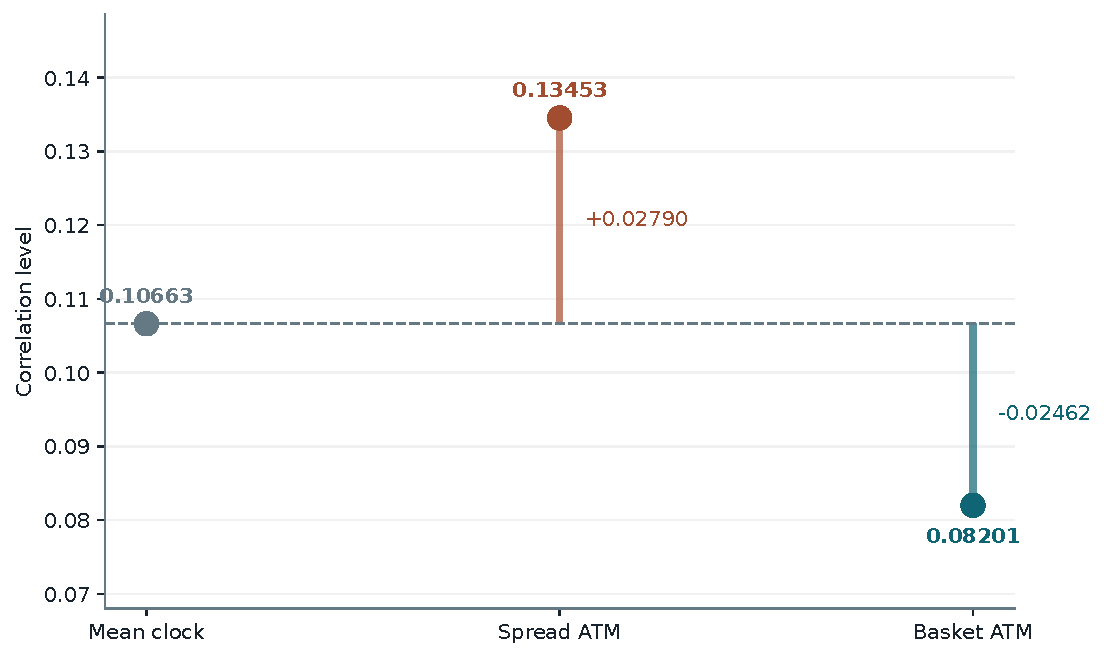
\includegraphics[width=0.82\linewidth,height=\textheight,keepaspectratio,alt={Point and stem plot showing mean clock correlation 0.10663, spread ATM implied correlation 0.13453, and basket ATM implied correlation 0.08201 with opposite Jensen corrections.}]{figures/vector/f02_atm_jensen_wedge.pdf}

}

\caption{\label{fig-atm-wedge}The exact ATM Jensen wedge for the
reference clock. The spread lies above the mean clock because its
correlation coefficient in total variance is negative; the basket lies
below because that coefficient is positive.}

\end{figure}%

\subsection{A small-dispersion
expansion}\label{a-small-dispersion-expansion}

The exact wedge is most informative, but a local approximation makes its
scale transparent. Write

\[
V_T=\bar v+\varepsilon,
\qquad
\bar v=E[V_T]>0,
\qquad
E[\varepsilon]=0.
\]

More precisely, consider a family

\[
V_T^{(\eta)}=\bar v+\eta\xi,
\qquad E[\xi]=0,
\qquad E[|\xi|^5]<\infty,
\]

and assume that for all sufficiently small \(|\eta|\) there is a fixed
\(r<1\) such that \(|\eta\xi|\le r\bar v\) almost surely. This uniform
separation from zero controls the Taylor remainder. With
\(\varepsilon=\eta\xi\),

\[
\sqrt{\bar v+\varepsilon}
=\sqrt{\bar v}
\left[
1+\frac{\varepsilon}{2\bar v}
-\frac{\varepsilon^2}{8\bar v^2}
+\frac{\varepsilon^3}{16\bar v^3}
-\frac{5\varepsilon^4}{128\bar v^4}
+O(\varepsilon^5)
\right].
\]

Taking expectations and squaring,

\begin{equation}\protect\phantomsection\label{eq-small-dispersion}{
(E[\sqrt{V_T}])^2
=\bar v
-\frac{E[\varepsilon^2]}{4\bar v}
+\frac{E[\varepsilon^3]}{8\bar v^2}
+\frac{E[\varepsilon^2]^2-5E[\varepsilon^4]}
{64\bar v^3}
+O(\eta^5).
}\end{equation}

For the correlation clock, keep the law of \(A_T\) fixed and let
\(\alpha\to0\). Then

\[
\bar v(\alpha)=\beta T+\alpha E[A_T],
\qquad
\varepsilon=\alpha(A_T-E[A_T]).
\]

Because \(A_T\) is bounded, the uniform-away-from-zero condition holds
for sufficiently small \(|\alpha|\). Dividing
Eq.~\ref{eq-small-dispersion} by \(\alpha T\) gives

\begin{equation}\protect\phantomsection\label{eq-wedge-expansion}{
\rho_{\mathrm{imp}}(0)-\bar\rho_T
=-\frac{\alpha\,\operatorname{Var}(A_T)}
{4T\bar v}
+\frac{\alpha^2E[(A_T-E[A_T])^3]}
{8T\bar v^2}
+O(|\alpha|^3).
}\end{equation}

The leading sign agrees with the exact theorem. The expansion should not
be used near a zero-variance boundary; the exact formula remains valid
there whenever the relevant moments exist.

\subsection{Numerical reconciliation}\label{numerical-reconciliation}

For Eq.~\ref{eq-reference-parameters}, deterministic Gaussian quadrature
gives

\[
E[A_T]=0.106628721753,
\qquad
\operatorname{Var}(A_T)=0.111738386500.
\]

The clock-density calculation and direct Bachelier inversion give:

\begin{longtable}[]{@{}
  >{\raggedright\arraybackslash}p{(\linewidth - 10\tabcolsep) * \real{0.1304}}
  >{\raggedleft\arraybackslash}p{(\linewidth - 10\tabcolsep) * \real{0.1739}}
  >{\raggedleft\arraybackslash}p{(\linewidth - 10\tabcolsep) * \real{0.1739}}
  >{\raggedleft\arraybackslash}p{(\linewidth - 10\tabcolsep) * \real{0.1739}}
  >{\raggedleft\arraybackslash}p{(\linewidth - 10\tabcolsep) * \real{0.1739}}
  >{\raggedleft\arraybackslash}p{(\linewidth - 10\tabcolsep) * \real{0.1739}}@{}}
\caption{Exact reference-clock ATM identities. Values are generated from
the bounded clock density and are not
fitted.}\label{tbl-atm-identities}\tabularnewline
\toprule\noalign{}
\begin{minipage}[b]{\linewidth}\raggedright
Case
\end{minipage} & \begin{minipage}[b]{\linewidth}\raggedleft
\(\alpha\)
\end{minipage} & \begin{minipage}[b]{\linewidth}\raggedleft
\(E[\sqrt{V_T}]\)
\end{minipage} & \begin{minipage}[b]{\linewidth}\raggedleft
\(\rho_{\mathrm{imp}}(0)\)
\end{minipage} & \begin{minipage}[b]{\linewidth}\raggedleft
\(\rho_{\mathrm{imp}}(0)-E[A_T]\)
\end{minipage} & \begin{minipage}[b]{\linewidth}\raggedleft
\(\rho_{\mathrm{imp}}''(0)\)
\end{minipage} \\
\midrule\noalign{}
\endfirsthead
\toprule\noalign{}
\begin{minipage}[b]{\linewidth}\raggedright
Case
\end{minipage} & \begin{minipage}[b]{\linewidth}\raggedleft
\(\alpha\)
\end{minipage} & \begin{minipage}[b]{\linewidth}\raggedleft
\(E[\sqrt{V_T}]\)
\end{minipage} & \begin{minipage}[b]{\linewidth}\raggedleft
\(\rho_{\mathrm{imp}}(0)\)
\end{minipage} & \begin{minipage}[b]{\linewidth}\raggedleft
\(\rho_{\mathrm{imp}}(0)-E[A_T]\)
\end{minipage} & \begin{minipage}[b]{\linewidth}\raggedleft
\(\rho_{\mathrm{imp}}''(0)\)
\end{minipage} \\
\midrule\noalign{}
\endhead
\bottomrule\noalign{}
\endlastfoot
Spread & \(-7.5\) & 2.73697 & 0.13453 & +0.02790 & -0.00799 \\
Basket & \(+7.5\) & 3.01912 & 0.08201 & -0.02462 & +0.00616 \\
\end{longtable}

The production density uses 160 Fourier modes, 2,001 clock points, and a
1,600-point localized factor grid. Its mean and variance differ from
independent Gaussian quadrature by \(1.45\times10^{-6}\) and
\(8.81\times10^{-7}\), respectively. A separate 192-mode, 2,400-point
audit moved the reported ATM correlations by at most
\(1.2\times10^{-6}\) and the curvatures by less than
\(2.0\times10^{-7}\). The table is therefore limited to the digits
supported by grid convergence; density normalization alone is not used
as a convergence test.

The spread and basket corrections have unequal magnitudes because
\(\sqrt{\beta T-\lvert\alpha\rvert A_T}\) and
\(\sqrt{\beta T+\lvert\alpha\rvert A_T}\) have different variances.

Figure~\ref{fig-curvature} illustrates the exact sign mechanism on a
transparent two-point family \(S\in\{e^{-a},e^a\}\) with equal
probabilities. In that family

\[
E[S]E[S^{-1}]-1
=\sinh^2a,
\]

so the implied-correlation curvatures are \(2\sinh^2a/(\alpha T)\). The
figure is a theorem illustration, not a calibration.

\begin{figure}[tbp]

\centering{

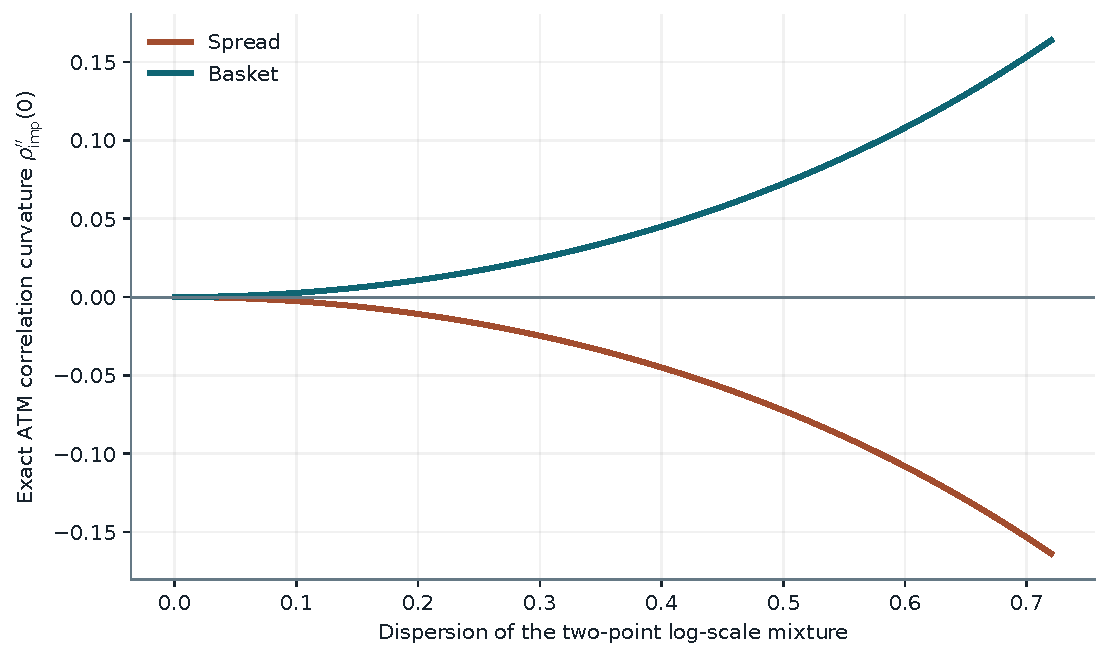
\includegraphics[width=0.82\linewidth,height=\textheight,keepaspectratio,alt={Two smooth curves starting at zero and diverging symmetrically: positive basket ATM correlation curvature and negative spread curvature as mixture dispersion increases.}]{figures/vector/f03_local_curvature.pdf}

}

\caption{\label{fig-curvature}Exact local implied-correlation curvature
for an equal-weight two-point log-scale mixture. Dispersion raises the
nonnegative curvature numerator; the sign of the correlation curvature
is then determined solely by the sign of the variance loading alpha.}

\end{figure}%

\subsection{What the theorem does not
imply}\label{what-the-theorem-does-not-imply}

The result is local at \(k=0\). It proves:

\begin{itemize}
\tightlist
\item
  exact smile evenness for a centered scale mixture;
\item
  the exact ATM level;
\item
  the existence and sign of finite ATM curvature under an inverse-moment
  condition; and
\item
  the exact translation into correlation units.
\end{itemize}

It does \textbf{not} prove that curvature retains one sign at every
strike, that the wings are monotone, or that every symmetric
distribution is a Gaussian scale mixture. Global wing behavior depends
on the complete mixing law.

The theorem also fails in its present form when the conditional mean is
random. That is precisely what Brownian leverage produces, and it is the
subject of Section Section~\ref{sec-leverage}.

\section{Leverage and one-dimensional transform
closure}\label{sec-leverage}

\subsection{Admissible Brownian
geometry}\label{admissible-brownian-geometry}

Remove the independence assumption between the factor driver and the
primitive asset drivers, retaining

\[
d[W^1,W^2]_t=0,\qquad
d[W^0,W^1]_t=\ell_1\,dt,\qquad
d[W^0,W^2]_t=\ell_2\,dt.
\]

In the coordinate order \((W^1,W^2,W^0)\), the Brownian correlation
matrix is

\begin{equation}\protect\phantomsection\label{eq-brownian-correlation}{
\Sigma_W=
\begin{pmatrix}
1&0&\ell_1\\
0&1&\ell_2\\
\ell_1&\ell_2&1
\end{pmatrix}.
}\end{equation}

\begin{lemma}[Admissible primitive leverage
region]\protect\hypertarget{lem-leverage-psd}{}\label{lem-leverage-psd}

The Brownian system Eq.~\ref{eq-brownian-correlation} exists if and only
if

\begin{equation}\protect\phantomsection\label{eq-leverage-disc}{
\boxed{\ell_1^2+\ell_2^2\le1.}
}\end{equation}

\end{lemma}

\begin{proof}
The one-dimensional principal minors equal one. The nontrivial
two-dimensional principal minors are

\[
1,\qquad 1-\ell_1^2,\qquad 1-\ell_2^2,
\]

and

\[
\det\Sigma_W=1-\ell_1^2-\ell_2^2.
\]

Nonnegativity of the determinant implies nonnegativity of the two
leverage minors. Conversely, nonnegativity of all principal minors is
sufficient for a symmetric matrix to be positive semidefinite.
\(\square\)
\end{proof}

Pairwise choices inside \([-1,1]\) are not enough. For example,
\((\ell_1,\ell_2)=(0.8,0.8)\) violates Eq.~\ref{eq-leverage-disc}.

Let \(\ell=(\ell_1,\ell_2)^\top\). Choose any matrix \(C\) such that

\begin{equation}\protect\phantomsection\label{eq-residual-root}{
CC^\top=I_2-\ell\ell^\top,
}\end{equation}

and let \(U=(U^1,U^2)\) be a two-dimensional Brownian motion independent
of \(W^0\). Then

\begin{equation}\protect\phantomsection\label{eq-orthogonal-decomposition}{
\begin{pmatrix}dW_t^1\\dW_t^2\end{pmatrix}
=\ell\,dW_t^0+C\,dU_t.
}\end{equation}

When \(|\ell_1|<1\), one explicit choice is

\[
dW_t^1
=\ell_1\,dW_t^0+\sqrt{1-\ell_1^2}\,dU_t^1,
\]

\begin{equation}\protect\phantomsection\label{eq-explicit-orthogonal}{
dW_t^2
=\ell_2\,dW_t^0
-\frac{\ell_1\ell_2}{\sqrt{1-\ell_1^2}}\,dU_t^1
+\sqrt{\frac{1-\ell_1^2-\ell_2^2}{1-\ell_1^2}}\,dU_t^2.
}\end{equation}

The construction preserves \(d[W^1,W^2]_t=0\). In particular, it
preserves the intended instantaneous asset correlation:

\[
\operatorname{Corr}(dF_{1,t},dF_{2,t}\mid\mathcal F_t)=f_c(X_t).
\]

The correlation between the factor and the second asset return is

\begin{equation}\protect\phantomsection\label{eq-state-dependent-second-leverage}{
\operatorname{Corr}
\left(
dW_t^0,\frac{dF_{2,t}}{\sigma_2}
\middle|\mathcal F_t
\right)
=\ell_1f_c(X_t)+\ell_2s_c(X_t),
}\end{equation}

so constant leverage against the primitive orthogonal drivers becomes
state-dependent leverage against the rotated second asset.

The instantaneous covariance-rate matrix of \((F_1,F_2,X)\) has
determinant

\begin{equation}\protect\phantomsection\label{eq-full-cov-determinant}{
\sigma_1^2\sigma_2^2\nu^2s_c(X_t)^2
\left(1-\ell_1^2-\ell_2^2\right)\ge0.
}\end{equation}

This determinant follows either by direct calculation or by taking the
squared determinant of the loading matrix times \(\det\Sigma_W\).

\subsection{Conditional Gaussianity with a random
mean}\label{conditional-gaussianity-with-a-random-mean}

For the linear combination Eq.~\ref{eq-linear-combination} define

\begin{equation}\protect\phantomsection\label{eq-g-loadings}{
g_1(x)=p+qf_c(x),
\qquad
g_2(x)=q s_c(x),
\qquad
g(x)=
\begin{pmatrix}g_1(x)\\g_2(x)\end{pmatrix}.
}\end{equation}

The component exposed to the factor Brownian motion is

\begin{equation}\protect\phantomsection\label{eq-common-loading}{
h(x)=\ell^\top g(x)
=\ell_1(p+qf_c(x))+\ell_2q s_c(x).
}\end{equation}

The residual loading and residual variance rate are

\[
r(x)=C^\top g(x),
\]

\begin{equation}\protect\phantomsection\label{eq-residual-variance}{
\Gamma(x)=\|r(x)\|^2
=g(x)^\top(I_2-\ell\ell^\top)g(x)
=Q(x)-h(x)^2\ge0.
}\end{equation}

Consequently,

\begin{equation}\protect\phantomsection\label{eq-leveraged-Z}{
dZ_t=h(X_t)\,dW_t^0+r(X_t)^\top dU_t.
}\end{equation}

\begin{theorem}[Leveraged conditional Gaussian
law]\protect\hypertarget{thm-conditional-leverage}{}\label{thm-conditional-leverage}

Conditional on the entire factor path,

\begin{equation}\protect\phantomsection\label{eq-leveraged-conditional-terminal}{
\boxed{
Z_T\mid X_{[0,T]}
\sim
N\left(
z_0+\int_0^Th(X_t)\,dW_t^0,\,
\int_0^T\Gamma(X_t)\,dt
\right).
}
}\end{equation}

More generally, the conditional process is Gaussian with mean curve

\[
m_t(X)=z_0+\int_0^th(X_s)\,dW_s^0
\]

and covariance

\begin{equation}\protect\phantomsection\label{eq-leveraged-conditional-covariance}{
\operatorname{Cov}(Z_s,Z_t\mid X)
=\int_0^{s\wedge t}\Gamma(X_r)\,dr.
}\end{equation}

\end{theorem}

\begin{proof}
The factor SDE Eq.~\ref{eq-factor} is invertible at path level:

\[
W_t^0=\frac{X_t-x_0-\mu t}{\nu}.
\]

Conditioning on \(X_{[0,T]}\) therefore conditions on \(W^0_{[0,T]}\).
The first term in Eq.~\ref{eq-leveraged-Z} is then fixed. The second is
an Itô integral against \(U\), which is independent of \(X\), with an
integrand that is deterministic under the conditional law. It is a
centered Gaussian process with covariance
Eq.~\ref{eq-leveraged-conditional-covariance}. \(\square\)
\end{proof}

The earlier claim that leverage ``destroys conditional Gaussianity''
confused centered conditional Gaussianity with conditional Gaussianity
itself. Independence is exactly the case \(h\equiv0\), for which the
conditional mean is \(z_0\) and the terminal law is a pure variance
mixture. Under leverage, the conditional mean is random.

This correction is consistent with established correlated mixing
formulas (Willard 1997; Alòs 2006; Das and Langrené 2022). The value
here is the explicit closure of the bounded-factor coefficients, not a
general discovery that correlated Brownian systems can be
orthogonalized.

\begin{figure}[tbp]

\centering{

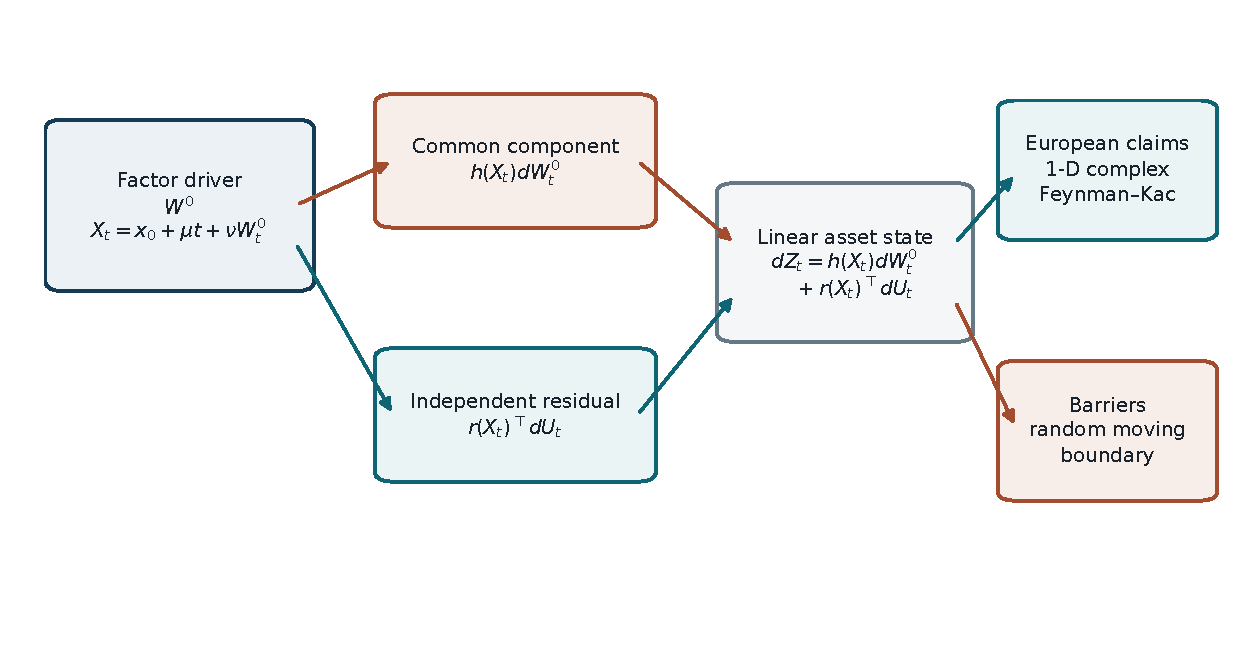
\includegraphics[width=1\linewidth,height=\textheight,keepaspectratio,alt={Flow diagram from factor Brownian motion to a common random conditional mean and an independent residual variance clock, which combine into a linear asset state and then branch to one-dimensional European transforms or moving-boundary barriers.}]{figures/vector/f04_leverage_geometry.pdf}

}

\caption{\label{fig-leverage-geometry}Orthogonal leverage decomposition.
Conditioning on the bounded-factor path fixes the common Brownian
component, leaving an independent Gaussian residual clock. Terminal
European claims retain one-dimensional transform closure, while barriers
inherit a random moving boundary.}

\end{figure}%

\subsection{An explicit Itô gauge}\label{an-explicit-ituxf4-gauge}

The stochastic integral in the conditional mean can be converted into an
endpoint and an ordinary additive functional. Let \(G'(x)=h(x)/\nu\).
Since

\[
\int f_c(x)\,dx=\sqrt{x^2+c^2},
\qquad
\int s_c(x)\,dx=c\,\operatorname{asinh}(x/c),
\]

an explicit primitive is

\begin{equation}\protect\phantomsection\label{eq-gauge-primitive}{
\boxed{
G(x)=\frac1\nu
\left[
\ell_1px
+q\ell_1\sqrt{x^2+c^2}
+q\ell_2c\,\operatorname{asinh}(x/c)
\right].
}
}\end{equation}

Moreover,

\begin{equation}\protect\phantomsection\label{eq-h-prime}{
h'(x)
=\frac{qc(\ell_1c-\ell_2x)}
{(x^2+c^2)^{3/2}}.
}\end{equation}

Define

\begin{equation}\protect\phantomsection\label{eq-gauge-K}{
K(x)
=\frac{\mu}{\nu}h(x)+\frac{\nu}{2}h'(x).
}\end{equation}

\begin{proposition}[Endpoint--additive gauge
identity]\protect\hypertarget{prp-ito-gauge}{}\label{prp-ito-gauge}

For every finite \(T\),

\begin{equation}\protect\phantomsection\label{eq-ito-gauge}{
\boxed{
\int_0^Th(X_t)\,dW_t^0
=G(X_T)-G(x_0)-\int_0^TK(X_t)\,dt.
}
}\end{equation}

Hence

\begin{equation}\protect\phantomsection\label{eq-gauged-conditional-law}{
Z_T\mid X
\sim
N\left(
z_0+G(X_T)-G(x_0)-\int_0^TK(X_t)\,dt,\,
\int_0^T\Gamma(X_t)\,dt
\right).
}\end{equation}

\end{proposition}

\begin{proof}
Apply Itô's formula:

\[
dG(X_t)
=G'(X_t)dX_t+\frac12G''(X_t)\nu^2dt.
\]

Using \(G'=h/\nu\), \(G''=h'/\nu\), and \(dX_t=\mu dt+\nu dW_t^0\),

\[
dG(X_t)
=h(X_t)dW_t^0
+\left[
\frac{\mu}{\nu}h(X_t)+\frac{\nu}{2}h'(X_t)
\right]dt.
\]

Integrate and rearrange. \(\square\)
\end{proof}

The inverse-hyperbolic-sine term is the distinctive consequence of
allowing the factor to load on the primitive orthogonal driver \(W^2\).
If \(\ell_2=0\), the primitive contains only a linear term and
\(\sqrt{x^2+c^2}\).

\subsection{One-dimensional transform
closure}\label{one-dimensional-transform-closure}

Let \(Y_t=Z_t-z_0\). The joint generator of \((X,Y)\) is

\begin{equation}\protect\phantomsection\label{eq-joint-generator}{
\mathcal L
=\mu\partial_x
+\frac{\nu^2}{2}\partial_{xx}
+\frac{Q(x)}{2}\partial_{yy}
+\nu h(x)\partial_{xy}.
}\end{equation}

Translation invariance in \(y\) is the structural reason that Fourier
transformation removes one state dimension.

\begin{theorem}[One-dimensional leveraged characteristic
transform]\protect\hypertarget{thm-leveraged-transform}{}\label{thm-leveraged-transform}

For \(u\in\mathbb R\), define

\[
v(\tau,x;u)
=E_{x,0}\left[e^{iuY_\tau}\right].
\]

Then \(v\) is the bounded solution of

\begin{equation}\protect\phantomsection\label{eq-complex-drift-pde}{
\boxed{
\partial_\tau v
=\frac{\nu^2}{2}v_{xx}
+\left(\mu+iu\nu h(x)\right)v_x
-\frac{u^2}{2}Q(x)v,
\qquad
v(0,x;u)=1.
}
}\end{equation}

The terminal characteristic function is

\begin{equation}\protect\phantomsection\label{eq-leveraged-cf}{
\boxed{
\phi_Z(u)=e^{iuz_0}v(T,x_0;u).
}
}\end{equation}

Equivalently, with the complex potential

\begin{equation}\protect\phantomsection\label{eq-complex-potential}{
\mathcal V_u(x)
=-iuK(x)-\frac{u^2}{2}\Gamma(x),
}\end{equation}

let

\[
w(\tau,x;u)
=E_x\left[
\exp\left(\int_0^\tau\mathcal V_u(X_s)\,ds\right)
e^{iuG(X_\tau)}
\right].
\]

Then

\begin{equation}\protect\phantomsection\label{eq-complex-potential-pde}{
\partial_\tau w
=\frac{\nu^2}{2}w_{xx}+\mu w_x+\mathcal V_u(x)w,
\qquad
w(0,x;u)=e^{iuG(x)},
}\end{equation}

and

\begin{equation}\protect\phantomsection\label{eq-gauged-cf}{
\boxed{
\phi_Z(u)
=e^{iu(z_0-G(x_0))}w(T,x_0;u).
}
}\end{equation}

\end{theorem}

\begin{proof}
For a Fourier mode \(e^{iuy}\psi(x)\),

\[
\partial_{yy}(e^{iuy}\psi)=-u^2e^{iuy}\psi,
\]

\[
\partial_{xy}(e^{iuy}\psi)=iu e^{iuy}\psi'(x).
\]

Apply the backward Kolmogorov equation for Eq.~\ref{eq-joint-generator}
and factor out \(e^{iuy}\) to obtain Eq.~\ref{eq-complex-drift-pde}.

For the second representation, take the conditional characteristic
function in Eq.~\ref{eq-gauged-conditional-law}:

\[
E[e^{iuZ_T}\mid X]
=
\exp\left\{
iu\left[
z_0+G(X_T)-G(x_0)-\int_0^TK(X_t)dt
\right]
-\frac{u^2}{2}\int_0^T\Gamma(X_t)dt
\right\}.
\]

Taking expectation over \(X\) gives Eq.~\ref{eq-gauged-cf}, and the
usual time-homogeneous Feynman--Kac theorem gives
Eq.~\ref{eq-complex-potential-pde}. \(\square\)
\end{proof}

When \(\ell=0\),

\[
h=G=K=0,\qquad \Gamma=Q,
\]

and both equations reduce to the real-potential variance-clock transform

\[
E\left[\exp\left(-\frac{u^2}{2}\int_0^TQ(X_t)dt\right)\right].
\]

The transform remains global. Because \(|f_c|\le1\),

\[
0\le Q(x)\le(|p|+|q|)^2.
\]

Thus

\[
[Y]_T=\int_0^TQ(X_t)dt
\le (|p|+|q|)^2T.
\]

\begin{corollary}[Sub-Gaussian exponential-moment
bound]\protect\hypertarget{cor-subgaussian}{}\label{cor-subgaussian}

For every real \(\theta\),

\begin{equation}\protect\phantomsection\label{eq-subgaussian-bound}{
E[e^{\theta Y_T}]
\le
\exp\left(
\frac{\theta^2}{2}(|p|+|q|)^2T
\right).
}\end{equation}

\end{corollary}

\begin{proof}
The Doléans exponential

\[
\exp\left(\theta Y_T-\frac{\theta^2}{2}[Y]_T\right)
\]

is a true martingale because the bracket is bounded. Therefore

\[
E[e^{\theta Y_T}]
=E\left[
\mathcal E(\theta Y)_T
e^{\theta^2[Y]_T/2}
\right]
\le e^{\theta^2(|p|+|q|)^2T/2}
E[\mathcal E(\theta Y)_T],
\]

and the last expectation equals one. \(\square\)
\end{proof}

Leverage-preserving transform closure is well known in affine and
correlated stochastic-volatility models (Heston 1993; Scott 1997; Duffie
et al. 2000). Theorem Theorem~\ref{thm-leveraged-transform} is valuable
because the bounded coefficients are nonaffine yet the Fourier reduction
and explicit gauge remain one-dimensional.

\subsection{Leverage creates skewness}\label{leverage-creates-skewness}

The independent model is a centered variance mixture and therefore
symmetric. Under leverage, the random conditional mean generically
breaks that symmetry.

\begin{proposition}[Short-time third
moment]\protect\hypertarget{prp-short-skew}{}\label{prp-short-skew}

Assume the coefficients are smooth near \(x_0\). Then

\begin{equation}\protect\phantomsection\label{eq-third-moment}{
\boxed{
E[Y_T^3]
=\frac32\nu h(x_0)Q'(x_0)T^2+o(T^2)
=3pq\nu h(x_0)f_c'(x_0)T^2+o(T^2).
}
}\end{equation}

\end{proposition}

\begin{proof}
From Eq.~\ref{eq-joint-generator},

\[
\mathcal L(y^3)=3yQ(x).
\]

At \((x_0,0)\) this is zero. Apply \(\mathcal L\) once more. Terms
carrying a factor \(y\) vanish at \(y=0\), and the cross derivative
contributes

\[
\mathcal L^2(y^3)\big|_{(x_0,0)}
=3\nu h(x_0)Q'(x_0).
\]

The short-time semigroup expansion gives

\[
E_{x_0,0}[Y_T^3]
=\frac{T^2}{2}
\mathcal L^2(y^3)\big|_{(x_0,0)}
+o(T^2).
\]

Finally, \(Q'(x)=2pqf_c'(x)\). \(\square\)
\end{proof}

If \(pq\,h(x_0)\ne0\), the third moment is nonzero at sufficiently small
maturity. This proves loss of exact symmetry but not necessarily a
nonzero ATM slope. For a continuous mean-zero terminal law with
Bachelier implied standard deviation \(I\),

\begin{equation}\protect\phantomsection\label{eq-general-atm-slope}{
I'(0)
=\frac{1/2-\mathbb P(Y_T>0)}{\varphi(0)}.
}\end{equation}

A skewed law can still have median zero. The distinction between
skewness, median displacement, and ATM slope must therefore be
preserved.

The leading coefficient in Eq.~\ref{eq-third-moment} is model-specific.
The general connection between leverage and option skew is established
in stochastic- volatility theory; it is not a new qualitative claim.

\subsection{Numerical transform check}\label{numerical-transform-check}

The deterministic evidence builder simulates the full correlated
Brownian system and compares it with both conditional representations.
Across 15 frequencies on \([0,2.8]\), the maximum
direct-versus-conditional gap is \(1.63\times10^{-3}\), below four
standard errors. The conditional-versus-gauge gap is
\(3.87\times10^{-5}\).

\begin{figure}[tbp]

\centering{

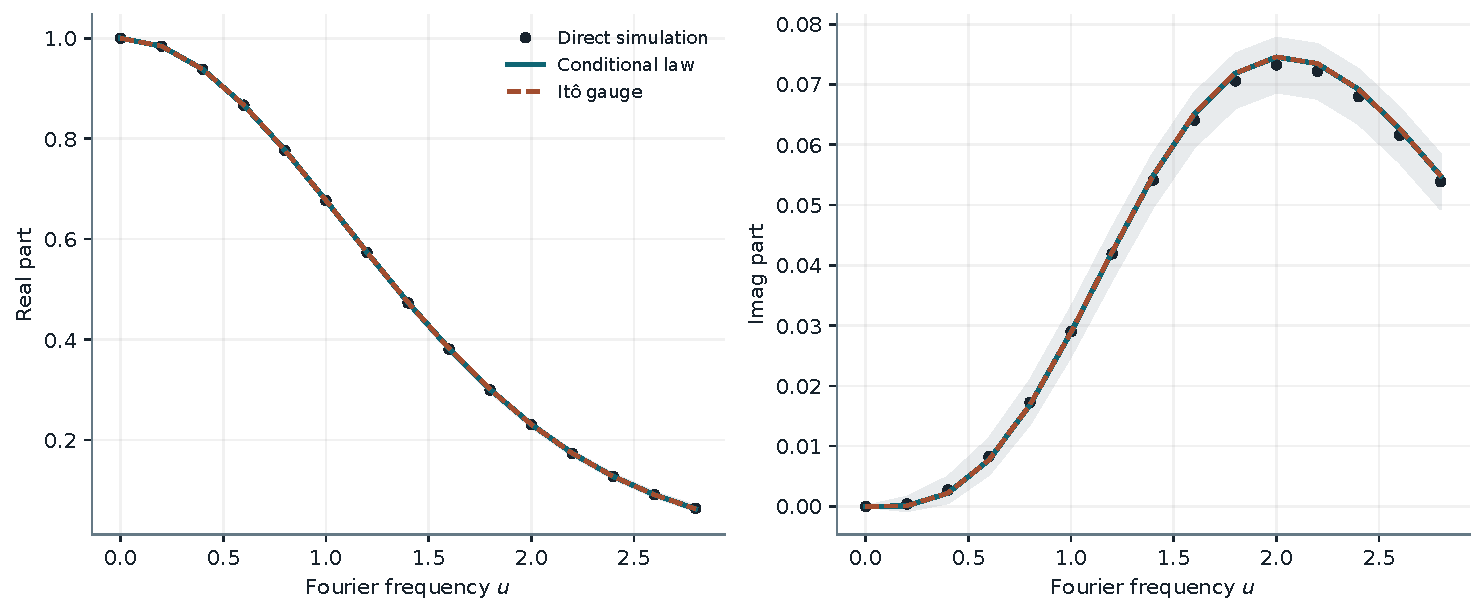
\includegraphics[width=1\linewidth,height=\textheight,keepaspectratio,alt={Two-panel plot of real and imaginary characteristic-function components. Direct simulation points overlap conditional-law and Ito-gauge curves across frequencies zero to 2.8.}]{figures/vector/f05_leverage_cf.pdf}

}

\caption{\label{fig-leverage-cf}Leveraged characteristic-function
validation. Direct simulation, conditional Gaussian integration, and the
Itô-gauge representation agree across Fourier frequencies; the shaded
band is two Monte Carlo standard errors around the direct estimate.}

\end{figure}%

\subsection{The true barrier frontier}\label{the-true-barrier-frontier}

Define

\[
M_t
=G(X_t)-G(x_0)-\int_0^tK(X_s)\,ds,
\qquad
J_t=\int_0^t\Gamma(X_s)\,ds.
\]

On an extension of the conditional probability space,

\begin{equation}\protect\phantomsection\label{eq-moving-boundary-representation}{
(Z_t\mid X)
\overset{d}{=}
(z_0+M_t+B_{J_t}\mid X),
}\end{equation}

where \(B\) is conditionally independent Brownian motion. For every
residual clock, the upper barrier event is

\begin{equation}\protect\phantomsection\label{eq-random-moving-boundary}{
\sup_{t\le T}
\left\{
B_{J_t}+M_t
\right\}
\ge d-z_0.
}\end{equation}

If \(\|\ell\|<1\) and \(Q(X_t)>0\), then \(I_2-\ell\ell^\top\) is
positive definite and \(J\) is strictly increasing. In that case
Eq.~\ref{eq-random-moving-boundary} can be rewritten as

\begin{equation}\protect\phantomsection\label{eq-strict-moving-boundary}{
\sup_{v\le J_T}
\left\{
B_v+M_{J^{-1}(v)}
\right\}
\ge d-z_0.
}\end{equation}

If \(J\) has flat intervals, Eq.~\ref{eq-random-moving-boundary} is the
canonical representation; no single-valued inverse-clock mean is
available in general. The event depends on the entire factor path, not
only \(J_T\). Thus the standard terminal scalar-clock reflection
derivation does not extend automatically; additional structure is
required. When \(h\equiv0\), the moving mean vanishes and the original
scalar-clock reduction is recovered.

This boundary is specific. Correlated stochastic-volatility barrier
formulas can exist under other multiplicative structures (Rolloos 2022).
The open classification problem is to identify nonzero \(h\) and
strictly increasing residual clocks for which \(M_{J^{-1}(v)}\) belongs
to a solvable moving- boundary family, together with degenerate-clock
cases solvable directly in calendar time.

\section{Phase-Gram quotient theory}\label{sec-phasegram}

\subsection{Triangular angles and the observable
quotient}\label{triangular-angles-and-the-observable-quotient}

The parameterization Eq.~\ref{eq-gram-factor} is an established way to
turn unconstrained angles into a valid correlation matrix (Pinheiro and
Bates 1996; Rebonato and Jäckel 2000; Rapisarda et al. 2007). Static
versions are widely used for optimization, simulation, and prior
construction (Joe 2006; Lewandowski et al. 2009; Pourahmadi and Wang
2015; Forrester and Zhang 2020).

The dynamic specification Eq.~\ref{eq-angle-bm} is deliberately simple:
independent unwrapped Brownian angles. The angle lift is Markov on
\(\mathbb R^d\) but has no invariant probability law there. The
observable matrix depends only on sines and cosines. It therefore
factors through a compact torus.

Write the closed elliptope as

\[
\mathcal E_n
=\left\{
R\in\mathbb S_+^n:
\operatorname{diag}(R)=\mathbf1
\right\}.
\]

Write

\[
\Theta_t
=(\theta_1(t),\ldots,\theta_d(t))
\pmod{2\pi}
\in\mathbb T^d.
\]

The wrapped coordinate process has generator

\[
\mathcal L_{\mathbb T}
=\frac12\sum_{j=1}^d\sigma_j^2\partial_{\theta_j\theta_j}.
\]

Product Haar measure on \(\mathbb T^d\) is invariant. ``Haar'' refers to
this coordinate torus; the elliptope of correlation matrices is not a
group and has no Haar probability measure.

\subsection{Exact determinant
factorization}\label{exact-determinant-factorization}

\begin{theorem}[Phase-Gram determinant and finite-time
moments]\protect\hypertarget{thm-phasegram-determinant}{}\label{thm-phasegram-determinant}

For every angle configuration,

\begin{equation}\protect\phantomsection\label{eq-det-factorization}{
\boxed{
\det R_t
=\prod_{j=1}^d\sin^2\theta_j(t).
}
}\end{equation}

Assume deterministic initial angles. For every positive integer \(m\),

\begin{equation}\protect\phantomsection\label{eq-det-moment-product}{
\boxed{
E[(\det R_t)^m]
=\prod_{j=1}^dM_{m,j}(t),
}
}\end{equation}

where

\begin{equation}\protect\phantomsection\label{eq-single-angle-moment}{
\boxed{
M_{m,j}(t)
=\frac1{4^m}\binom{2m}{m}
+\frac{2}{4^m}
\sum_{r=1}^m
(-1)^r
\binom{2m}{m-r}
e^{-2r^2\sigma_j^2t}
\cos(2r\theta_j(0)).
}
}\end{equation}

For a random initial vector independent of future Brownian increments,

\begin{equation}\protect\phantomsection\label{eq-random-start-moment}{
E[(\det R_t)^m]
=E\left[\prod_{j=1}^d
M_{m,j}(t;\theta_j(0))\right].
}\end{equation}

\end{theorem}

\begin{proof}
The Gram factor is lower triangular, so

\[
\det R=(\det B)^2
=\prod_{i=2}^nB_{ii}^2.
\]

By Eq.~\ref{eq-gram-factor},

\[
B_{ii}^2
=\prod_{k<i}\sin^2\theta_{ik},
\]

and every one of the \(d=n(n-1)/2\) angles appears once. This proves
Eq.~\ref{eq-det-factorization}.

For an integer \(m\ge1\),

\begin{equation}\protect\phantomsection\label{eq-sine-power-fourier}{
\sin^{2m}x
=\frac1{4^m}\binom{2m}{m}
+\frac2{4^m}
\sum_{r=1}^m
(-1)^r\binom{2m}{m-r}\cos(2rx).
}\end{equation}

Since

\[
E[\cos(2r\theta_j(t))]
=e^{-2r^2\sigma_j^2t}\cos(2r\theta_j(0)),
\]

the expectation of \(\sin^{2m}\theta_j(t)\) is
Eq.~\ref{eq-single-angle-moment}. Deterministic initial angles and
independent drivers make the terminal angles independent, producing
Eq.~\ref{eq-det-moment-product}. Conditioning on a random initial vector
gives Eq.~\ref{eq-random-start-moment}. \(\square\)
\end{proof}

The determinant factorization itself is classical in hyperspherical
coordinates (Pourahmadi and Wang 2015; Forrester and Zhang 2020), as are
product- distribution techniques (Springer and Thompson 1970; Tang and
Gupta 1984). The dynamic content in
Theorem~\ref{thm-phasegram-determinant} is the explicit finite-time
Fourier damping for the Brownian angles.

For \(m=1\),

\begin{equation}\protect\phantomsection\label{eq-first-det-moment}{
E[\det R_t]
=\prod_{j=1}^d
\frac{1-e^{-2\sigma_j^2t}\cos(2\theta_j(0))}{2}.
}\end{equation}

Figure~\ref{fig-phasegram-moments} compares the first two exact moments
with independent terminal-angle simulation.

\begin{figure}[tbp]

\centering{

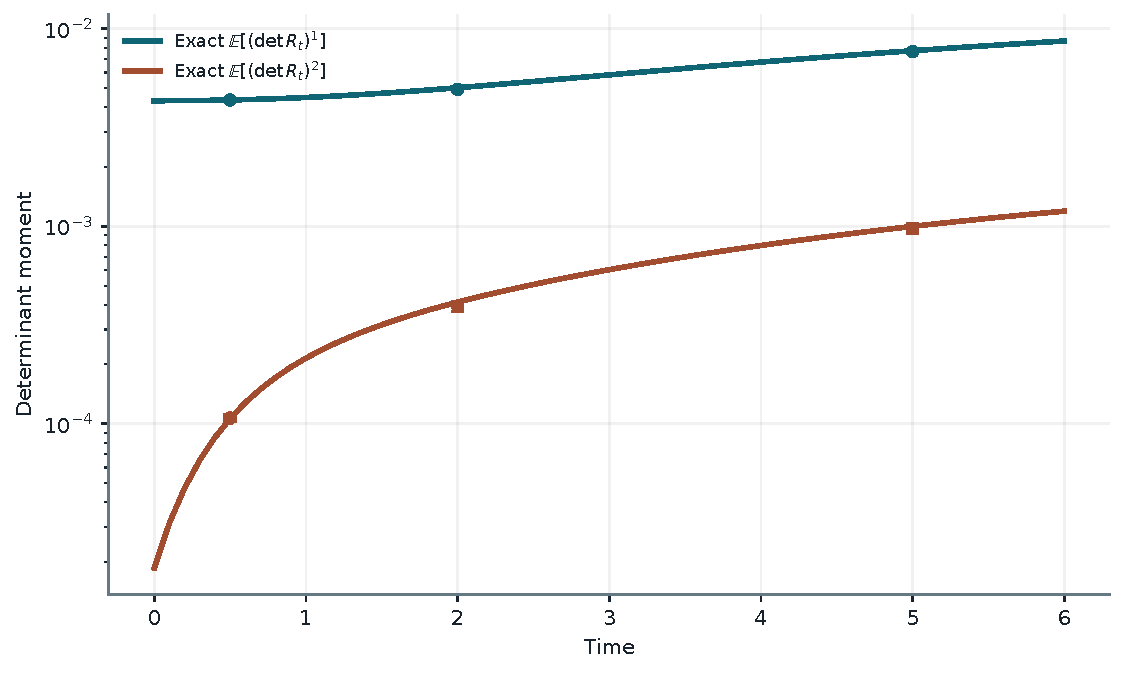
\includegraphics[width=0.84\linewidth,height=\textheight,keepaspectratio,alt={Log-scale plot of first and second determinant moments over time. Exact teal and rust curves pass through Monte Carlo points with small error bars.}]{figures/vector/f06_phasegram_moments.pdf}

}

\caption{\label{fig-phasegram-moments}Exact finite-time Phase-Gram
determinant moments. Solid curves are the finite Fourier formulas;
points with two-standard-error bars are independent Monte Carlo checks.}

\end{figure}%

\subsection{Compact stationarity}\label{compact-stationarity}

For one coordinate, Brownian motion modulo \(2\pi\) has transition
density

\begin{equation}\protect\phantomsection\label{eq-wrapped-heat-kernel}{
p_t(\theta\mid\theta_0)
=\frac1{2\pi}
\left[
1+2\sum_{k=1}^\infty
e^{-k^2\sigma^2t/2}
\cos(k(\theta-\theta_0))
\right].
}\end{equation}

The nonconstant Fourier modes decay exponentially. The product process
on \(\mathbb T^d\) therefore converges to product-uniform measure. This
is a special case of Brownian and Lévy convergence on compact groups
(Applebaum 2014; Liao 2004; Maher 2012).

\begin{theorem}[Stationary matrix pushforward
law]\protect\hypertarget{thm-phasegram-stationary}{}\label{thm-phasegram-stationary}

Let \(U_1,\ldots,U_d\) be independent uniform random variables on
\([0,2\pi)\) and define

\[
\Pi_n=\operatorname{Law}(R(U_1,\ldots,U_d)).
\]

Then, for every deterministic initial angle vector,

\begin{equation}\protect\phantomsection\label{eq-matrix-convergence}{
\boxed{
R_t\Longrightarrow\Pi_n
\qquad(t\to\infty).
}
}\end{equation}

If the wrapped initial angles are independent uniform variables
independent of the Brownian drivers, the matrix process is strictly
stationary. Its mean is

\begin{equation}\protect\phantomsection\label{eq-stationary-mean}{
\boxed{
E_{\Pi_n}[R]=I_n.
}
}\end{equation}

\end{theorem}

\begin{proof}
Equation Eq.~\ref{eq-wrapped-heat-kernel} and independence give weak
convergence of \(\Theta_t\) to product Haar measure on \(\mathbb T^d\).
The Gram map is continuous and periodic, so the continuous-mapping
theorem gives Eq.~\ref{eq-matrix-convergence}.

Under product-uniform initialization, the wrapped angle process is
stationary, and every finite-dimensional matrix law obtained by applying
\(R(\cdot)\) is stationary.

For the mean, rows belonging to different asset indices depend on
disjoint angle sets and are independent. Every coordinate of a nonfirst
row contains either a cosine with zero uniform mean or a product
containing at least one sine with zero mean. Hence each nonfirst row has
mean zero. Off-diagonal Gram entries have zero expectation; diagonal
entries equal one pathwise. \(\square\)
\end{proof}

The conclusion is about matrix marginals and stationary
finite-dimensional laws. It does not automatically imply that the image
process \(R_t\) is Markov on the elliptope: a measurable image of a
Markov process need not be Markov. Away from singular fibers the
canonical chart is locally invertible; behavior at the boundary is the
unresolved point.

The correct long-horizon statement is therefore:

\begin{quote}
The unwrapped coordinates continue to diffuse, while the observable
matrix marginals converge to a compact stationary pushforward law.
\end{quote}

The path continues to accumulate quadratic variation and, as shown
below, hits the boundary recurrently.

\subsection{The invariant law is not uniform and not
LKJ}\label{the-invariant-law-is-not-uniform-and-not-lkj}

In the canonical interior chart \(0<\theta_{jk}<\pi\), the absolute
Jacobian from angles to off-diagonal correlations is

\begin{equation}\protect\phantomsection\label{eq-angle-jacobian}{
J(\theta)
=\prod_{k=1}^{n-1}
\prod_{j=k+1}^n
\sin^{\,n-k}\theta_{jk}.
}\end{equation}

This Jacobian underlies classical elliptope-volume and
random-correlation calculations (Pourahmadi and Wang 2015; Forrester and
Zhang 2020; Eastman et al. 2016; Muirhead 1982). Passing from the
unwrapped factor to the unique positive-diagonal canonical chart
requires a joint sign argument.

\begin{lemma}[Flat angles remain flat in the canonical
chart]\protect\hypertarget{lem-canonical-folding}{}\label{lem-canonical-folding}

Off the boundary, let

\[
D_{kk}=\operatorname{sgn}(B_{kk}),
\qquad
L=BD.
\]

Then \(LL^\top=BB^\top\), \(L\) has positive diagonal, and the canonical
angles of \(L\) are independent uniform variables on \((0,\pi)\) under
product-uniform unwrapped angles.

\end{lemma}

\begin{proof}
Since \(D^2=I\), right multiplication by \(D\) preserves the Gram matrix
and makes \(L_{kk}=|B_{kk}|>0\). Proceed row by row. Conditional on the
angles in earlier rows, the column signs \(D_{11},\ldots,D_{i-1,i-1}\)
are fixed and are independent of the row-\(i\) angles. The
product-uniform distribution of the hyperspherical row is invariant
under every coordinate sign flip: each flip is implemented by a
reflection or half-period shift of one of its uniform angles.
Multiplication by the fixed earlier column signs therefore preserves the
row law. The final sign \(D_{ii}=\operatorname{sgn}(B_{ii})\) folds the
last coordinate positive; its two equal-measure preimages produce a
uniform canonical angle on \((0,\pi)\). Almost everywhere, the map from
the row's \([0,2\pi)^{i-1}\) angles to its canonical \((0,\pi)^{i-1}\)
angles has \(2^{i-1}\) equal-measure reflection preimages, so its
pushforward density is \(\pi^{-(i-1)}\). Induction over \(i\) preserves
independence of all canonical angles and gives joint density
\(\pi^{-d}\). \(\square\)
\end{proof}

The canonical change-of-variables formula and
Lemma~\ref{lem-canonical-folding} therefore give the density of
\(\Pi_n\), with respect to Lebesgue measure on the off-diagonal
correlations and away from the boundary:

\begin{equation}\protect\phantomsection\label{eq-flat-angle-density}{
f_{\Pi_n}(R)
=\pi^{-d}J(\theta(R))^{-1}.
}\end{equation}

It is boundary-singular and depends on the triangular ordering. Here
``boundary-singular'' means the interior Lebesgue density is unbounded
when the boundary is approached; it does not mean that the invariant law
charges the boundary. In fact,

\[
\Pi_n(\partial\mathcal E_n)=0.
\]

By contrast, the LKJ family has

\[
f_{\operatorname{LKJ}(\eta)}(R)
\propto(\det R)^{\eta-1},
\]

whose canonical angle density is proportional to

\begin{equation}\protect\phantomsection\label{eq-lkj-angle-density}{
\prod_{k<j}
\sin^{\,2\eta+n-k-2}\theta_{jk}.
}\end{equation}

Flat angles cannot match one value of \(\eta\) for every \(k\) once
\(n\ge3\). For \(n=2\), flat angles correspond to
\(\operatorname{LKJ}(1/2)\), not the uniform \(\operatorname{LKJ}(1)\)
law (Joe 2006; Lewandowski et al. 2009).

The lack of permutation invariance is already visible at \(n=3\). With

\[
R_{12}=\cos\theta_{21},
\qquad
R_{13}=\cos\theta_{31},
\]

\[
R_{23}
=\cos\theta_{21}\cos\theta_{31}
+\sin\theta_{21}\sin\theta_{31}\cos\theta_{32},
\]

product-uniform angles give

\begin{equation}\protect\phantomsection\label{eq-ordering-moments}{
E[R_{12}^2]=E[R_{13}^2]=\frac12,
\qquad
E[R_{23}^2]=\frac38.
}\end{equation}

Thus \(E[R]=I\) hides heterogeneous entry marginals. There is no unique
``random correlation matrix'' baseline; different generation schemes
produce different geometries (Holmes 1991; Bendel and Mickey 1978;
Barnard et al. 2000; Archakov et al. 2024).

\subsection{Stationary determinant
law}\label{stationary-determinant-law}

Under \(\Pi_n\),

\[
Y_j=\sin^2U_j
\sim\operatorname{Beta}\left(\frac12,\frac12\right)
\]

independently. Consequently,

\begin{equation}\protect\phantomsection\label{eq-product-beta}{
\boxed{
\det R\overset d=\prod_{j=1}^dY_j.
}
}\end{equation}

\begin{corollary}[Mellin transform and log
cumulants]\protect\hypertarget{cor-phasegram-mellin}{}\label{cor-phasegram-mellin}

For \(\operatorname{Re}z>-1/2\),

\begin{equation}\protect\phantomsection\label{eq-det-mellin}{
\boxed{
E_{\Pi_n}[(\det R)^z]
=
\left[
\frac{\Gamma(z+\tfrac12)}
{\sqrt\pi\,\Gamma(z+1)}
\right]^d.
}
}\end{equation}

Moreover,

\begin{equation}\protect\phantomsection\label{eq-logdet-cumulants}{
\boxed{
E_{\Pi_n}[\log\det R]
=-2d\log2,
\qquad
\operatorname{Var}_{\Pi_n}(\log\det R)
=\frac{d\pi^2}{3}.
}
}\end{equation}

In particular,

\begin{equation}\protect\phantomsection\label{eq-det-means}{
E_{\Pi_n}[\det R]=2^{-d},
\qquad
\exp(E_{\Pi_n}[\log\det R])=4^{-d}.
}\end{equation}

\end{corollary}

\begin{proof}
For \(Y\sim\operatorname{Beta}(1/2,1/2)\),

\[
E[Y^z]
=\frac{B(z+\tfrac12,\tfrac12)}
{B(\tfrac12,\tfrac12)}
=\frac{\Gamma(z+\tfrac12)}
{\sqrt\pi\,\Gamma(z+1)}.
\]

Independence yields Eq.~\ref{eq-det-mellin}. Differentiate the log
Mellin transform at zero. The digamma identities

\[
\psi(1/2)-\psi(1)=-2\log2
\]

and trigamma identities

\[
\psi_1(1/2)-\psi_1(1)=\frac{\pi^2}{3}
\]

give Eq.~\ref{eq-logdet-cumulants}. Set \(z=1\) for the arithmetic
determinant mean. The geometric mean is the exponential of the log mean.
\(\square\)
\end{proof}

These Beta and polygamma facts are standard (Johnson et al. 1995). The
notable feature is their exact iid specialization under the flat-angle
invariant law. Determinant products and asymptotics also appear in
established Gram, Jacobi, and random-correlation ensembles (Rouault
2007; Hanea and Nane 2018); comparisons across ensembles are necessary
before declaring one unusually ill-conditioned.

\subsection{High-dimensional
asymptotics}\label{high-dimensional-asymptotics}

Let \(R_n\sim\Pi_n\) be coupled by one infinite iid sequence of
stationary angles and write \(d_n=n(n-1)/2\). Each increase in \(n\)
then adds independent \(\operatorname{Beta}(1/2,1/2)\) determinant
factors. The strong law gives

\begin{equation}\protect\phantomsection\label{eq-logdet-lln}{
\boxed{
\frac1{d_n}\log\det R_n
\longrightarrow-2\log2
\quad\text{almost surely}.
}
}\end{equation}

The central limit theorem gives

\begin{equation}\protect\phantomsection\label{eq-logdet-clt}{
\boxed{
\frac{\log\det R_n+2d_n\log2}
{\pi\sqrt{d_n/3}}
\Longrightarrow N(0,1).
}
}\end{equation}

Figure~\ref{fig-logdet} shows the finite-dimensional approach to the
normal limit. The \(n=3\) standardized law has a visible finite upper
endpoint because \(\log\det R_n\le0\); the boundary moves right as
\(d_n\) grows.

\begin{figure}[tbp]

\centering{

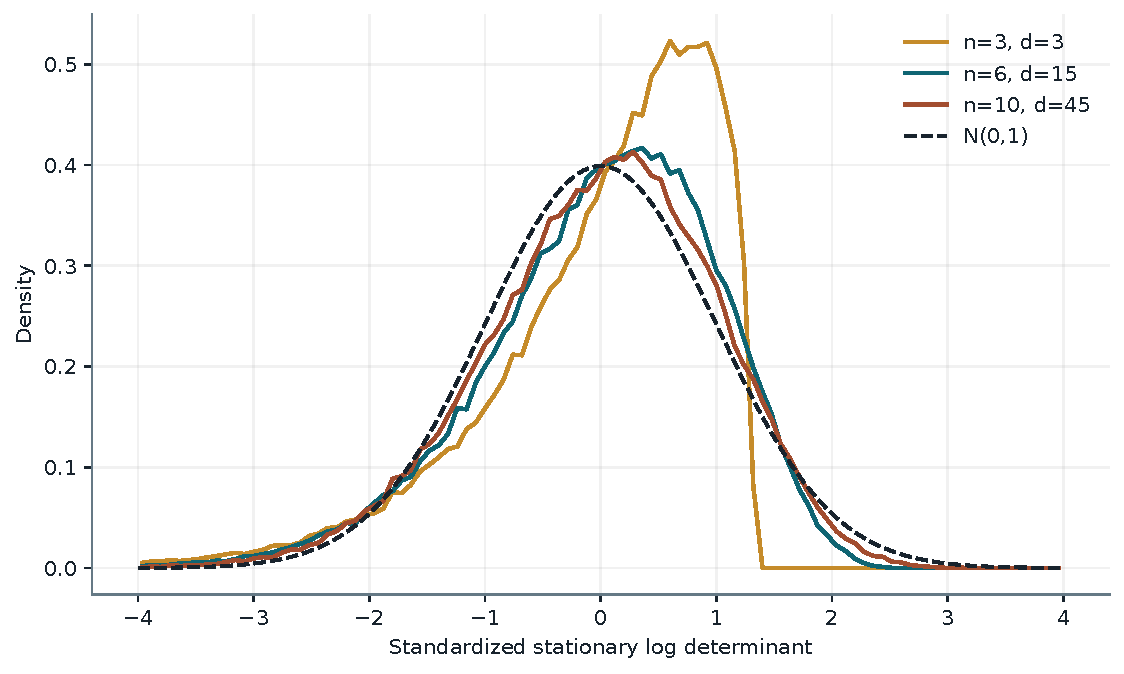
\includegraphics[width=0.84\linewidth,height=\textheight,keepaspectratio,alt={Density curves of standardized stationary log determinants for three, six, and ten assets compared with a dashed standard normal density. The curves become progressively closer to normal.}]{figures/vector/f07_phasegram_logdet.pdf}

}

\caption{\label{fig-logdet}Stationary Phase-Gram log-determinant
distributions after exact centering and scaling. The finite-dimensional
laws approach the standard normal reference as the number of independent
angular factors grows.}

\end{figure}%

Determinant decay yields a rigorous but one-sided eigenvalue
implication. For positive-definite \(R_n\),

\[
\lambda_{\min}(R_n)
\le(\det R_n)^{1/n}.
\]

Since \(2d_n=n(n-1)\), Eq.~\ref{eq-logdet-lln} implies the explicit
high-probability bound: for every \(\varepsilon>0\),

\begin{equation}\protect\phantomsection\label{eq-min-eigen-upper}{
\boxed{
\mathbb P\left(
\lambda_{\min}(R_n)
\le
2^{-(1-\varepsilon)(n-1)}
\right)
\longrightarrow1.
}
}\end{equation}

This is an upper bound, not a smallest-eigenvalue limit. Sharp
condition- number and eigenvalue laws remain open.

\subsection{First contact with the elliptope
boundary}\label{first-contact-with-the-elliptope-boundary}

Assume a deterministic interior initial angle vector:

\[
x_j=\theta_j(0)\pmod\pi\in(0,\pi).
\]

The determinant vanishes exactly when at least one angle hits a multiple
of \(\pi\). Let

\[
\tau_j
=\inf\{t>0:\theta_j(t)\notin(k_j\pi,(k_j+1)\pi)\},
\]

where the interval contains \(\theta_j(0)\), and let

\begin{equation}\protect\phantomsection\label{eq-first-singularity}{
\tau_\partial
=\inf\{t>0:\det R_t=0\}
=\min_{1\le j\le d}\tau_j.
}\end{equation}

The killed heat equation on \((0,\pi)\) gives the one-angle survival
probability

\begin{equation}\protect\phantomsection\label{eq-angle-survival}{
S_j(t)
=\frac4\pi
\sum_{m=0}^\infty
\frac{\sin((2m+1)x_j)}{2m+1}
\exp\left[
-\frac12(2m+1)^2\sigma_j^2t
\right].
}\end{equation}

This is the standard odd sine-series solution for Brownian interval exit
(Karatzas and Shreve 1991; Borodin and Salminen 2002).

\begin{theorem}[Exact first-singularity survival
law]\protect\hypertarget{thm-first-singularity}{}\label{thm-first-singularity}

For deterministic interior initial angles,

\begin{equation}\protect\phantomsection\label{eq-singularity-survival}{
\boxed{
\mathbb P(\tau_\partial>t)
=\prod_{j=1}^dS_j(t).
}
}\end{equation}

In particular, \(\tau_\partial<\infty\) almost surely, and the matrix
hits the boundary infinitely often.

If the initial angle vector is random but independent of future Brownian
increments,

\begin{equation}\protect\phantomsection\label{eq-random-singularity-survival}{
\mathbb P(\tau_\partial>t)
=E\left[
\prod_{j=1}^d
S(t;\theta_j(0)\bmod\pi,\sigma_j)
\right].
}\end{equation}

\end{theorem}

\begin{proof}
Equation Eq.~\ref{eq-det-factorization} gives

\[
\{\tau_\partial>t\}
=\bigcap_{j=1}^d\{\tau_j>t\}.
\]

With deterministic starts, the exit times are independent because the
angle drivers are independent. Multiply their survival probabilities.
Each one-dimensional Brownian motion exits a finite interval almost
surely, so the minimum does also. Brownian recurrence gives infinitely
many subsequent hits of \(\pi\mathbb Z\). Conditioning on a random
initial vector gives Eq.~\ref{eq-random-singularity-survival}.
\(\square\)
\end{proof}

At every fixed deterministic \(t>0\), the angle distribution is
continuous, so the probability of exact singularity is zero and \(R_t\)
is positive definite almost surely. Pathwise, however, the matrix
repeatedly leaves and re-enters the interior. Stationarity and recurrent
boundary contact are therefore compatible.

The killed-heat formula Eq.~\ref{eq-angle-survival} is classical. The
model-specific step is the determinant-factorization reduction of the
first matrix singularity to the minimum of independent interval exits;
no novelty is claimed for the sine-series heat solution itself.

\section{Corrected and extended exactness
frontiers}\label{sec-frontiers}

\subsection{Nonautonomous Feynman--Kac is an ordering
problem}\label{sec-nonautonomous}

Let

\[
\mathcal A_t=\mathcal L_t+\mathcal V_t
\]

be a time-dependent tilted generator. For a terminal payoff \(g\),
define the two-time evolution family

\begin{equation}\protect\phantomsection\label{eq-evolution-family}{
Q_{s,t}g(x)
=E_{s,x}\left[
\exp\left(\int_s^t\mathcal V_r(X_r)\,dr\right)
g(X_t)
\right].
}\end{equation}

Under the usual well-posedness, domain, and regularity hypotheses, the
standard two-time backward Feynman--Kac theorem remains valid:

\begin{equation}\protect\phantomsection\label{eq-two-time-backward}{
\boxed{
-\partial_sQ_{s,t}
=\mathcal A_sQ_{s,t},
\qquad
Q_{t,t}=I.
}
}\end{equation}

Time-dependent Feynman--Kac formulas and two-parameter evolution
operators are classical (Kac 1949; Karatzas and Shreve 1991; Kato 1953;
Pazy 1983; Acquistapace and Terreni 1987; Lunardi 1995). The issue
arises when the terminal time is varied while the initial calendar time
remains fixed. The correct terminal derivative is a \textbf{right
action}:

\begin{equation}\protect\phantomsection\label{eq-right-action}{
\boxed{
\partial_tQ_{0,t}=Q_{0,t}\mathcal A_t.
}
}\end{equation}

It is generally not \(\mathcal A_tQ_{0,t}\).

\begin{theorem}[Exact operator-ordering
defect]\protect\hypertarget{thm-commutator-defect}{}\label{thm-commutator-defect}

On a common invariant core on which the displayed products are defined
and strongly differentiable,

\begin{equation}\protect\phantomsection\label{eq-commutator-defect}{
\boxed{
(\partial_t-\mathcal A_t)Q_{0,t}g
=[Q_{0,t},\mathcal A_t]g
=\int_0^t
Q_{0,r}
[\mathcal A_r,\mathcal A_t]
Q_{r,t}g\,dr,
}
}\end{equation}

where \([B,C]=BC-CB\).

\end{theorem}

\begin{proof}
The first equality is Eq.~\ref{eq-right-action}. For the second, fix
\(t\) and define

\[
F(r)=Q_{0,r}\mathcal A_tQ_{r,t}.
\]

Using

\[
\partial_rQ_{0,r}=Q_{0,r}\mathcal A_r,
\qquad
\partial_rQ_{r,t}=-\mathcal A_rQ_{r,t},
\]

we obtain

\[
F'(r)
=Q_{0,r}
(\mathcal A_r\mathcal A_t-\mathcal A_t\mathcal A_r)
Q_{r,t}
=Q_{0,r}[\mathcal A_r,\mathcal A_t]Q_{r,t}.
\]

At the endpoints,

\[
F(t)=Q_{0,t}\mathcal A_t,
\qquad
F(0)=\mathcal A_tQ_{0,t}.
\]

Integrate from zero to \(t\). \(\square\)
\end{proof}

Pairwise commutation is sufficient for the naive horizon equation. The
integrated identity does not justify a general converse. Time ordering
and commutator expansions are central in the Magnus literature (Magnus
1954; Blanes et al. 2009); no novelty is claimed for the operator
calculus.

\subsubsection{A complete Gaussian
diagnostic}\label{a-complete-gaussian-diagnostic}

Fix \(T_*>0\) and consider deterministic curves satisfying

\[
\mu\in L^1([0,T_*]),
\qquad
\sigma\in L^2([0,T_*]),
\]

with dynamics

\[
dX_t=\mu(t)\,dt+\sigma(t)\,dW_t,
\qquad X_0=x,
\]

and the linear additive functional

\[
\mathcal J_T=\int_0^TX_s\,ds.
\]

Stochastic Fubini gives

\begin{equation}\protect\phantomsection\label{eq-integrated-gaussian}{
\mathcal J_T
=xT
+\int_0^T(T-r)\mu(r)\,dr
+\int_0^T(T-r)\sigma(r)\,dW_r.
}\end{equation}

Therefore, for real \(\lambda\),

\begin{equation}\protect\phantomsection\label{eq-true-nonautonomous}{
\boxed{
E_x[e^{\lambda\mathcal J_T}]
=
\exp\left\{
\lambda\left[
xT+\int_0^T(T-r)\mu(r)\,dr
\right]
+\frac{\lambda^2}{2}
\int_0^T(T-r)^2\sigma(r)^2\,dr
\right\}.
}
}\end{equation}

The misordered initial-value equation

\begin{equation}\protect\phantomsection\label{eq-misordered-pde}{
\partial_Tu
=\mu(T)u_x+\frac12\sigma(T)^2u_{xx}
+\lambda xu,
\qquad
u(0,x)=1,
}\end{equation}

instead yields

\begin{equation}\protect\phantomsection\label{eq-misordered-transform}{
\boxed{
\widetilde u(T,x)
=
\exp\left\{
\lambda\left[
xT+\int_0^Tr\mu(r)\,dr
\right]
+\frac{\lambda^2}{2}
\int_0^Tr^2\sigma(r)^2\,dr
\right\}.
}
}\end{equation}

\begin{proposition}[Constant-coefficient iff for the linear-potential
diagnostic]\protect\hypertarget{prp-linear-classification}{}\label{prp-linear-classification}

The transforms Eq.~\ref{eq-true-nonautonomous} and
Eq.~\ref{eq-misordered-transform} agree for every \(T\in(0,T_*]\) and
every \(\lambda\) if and only if \(\mu(t)\) and \(\sigma(t)^2\) are
constant almost everywhere on \((0,T_*]\).

\end{proposition}

\begin{proof}
Equality of the coefficients of \(\lambda\) and \(\lambda^2\) requires,
for \(a=\mu\) and for \(a=\sigma^2\),

\begin{equation}\protect\phantomsection\label{eq-centroid-identity}{
T\int_0^Ta(r)\,dr
=2\int_0^Tra(r)\,dr
}\end{equation}

for every \(T\in(0,T_*]\). Let \(A(T)=\int_0^Ta(r)\,dr\). Then

\[
TA(T)=2\int_0^Tra(r)\,dr.
\]

Differentiate almost everywhere:

\[
A(T)+Ta(T)=2Ta(T),
\]

so \(A(T)=Ta(T)\). Since \(A'=a\),

\[
A'(T)=\frac{A(T)}{T}
\]

almost everywhere on \((0,T_*]\). Hence \(A(T)=cT\) and \(a(T)=c\)
almost everywhere on that interval. Constants plainly satisfy
Eq.~\ref{eq-centroid-identity}. \(\square\)
\end{proof}

The proper backward solution retains both calendar times:

\[
u(s,x;T)
=\exp\left\{
\lambda\left[
(T-s)x+\int_s^T(T-r)\mu(r)\,dr
\right]
+\frac{\lambda^2}{2}
\int_s^T(T-r)^2\sigma(r)^2\,dr
\right\},
\]

and satisfies

\[
\partial_su+\mathcal A_su=0,
\qquad
u(T,x;T)=1.
\]

Figure~\ref{fig-operator-order} displays the ordering and the
quantitative divergence for \(\mu(t)=t\), \(\sigma(t)^2=1+t\),
\(x=0.2\), and \(\lambda=0.7\).

\begin{figure}[tbp]

\centering{

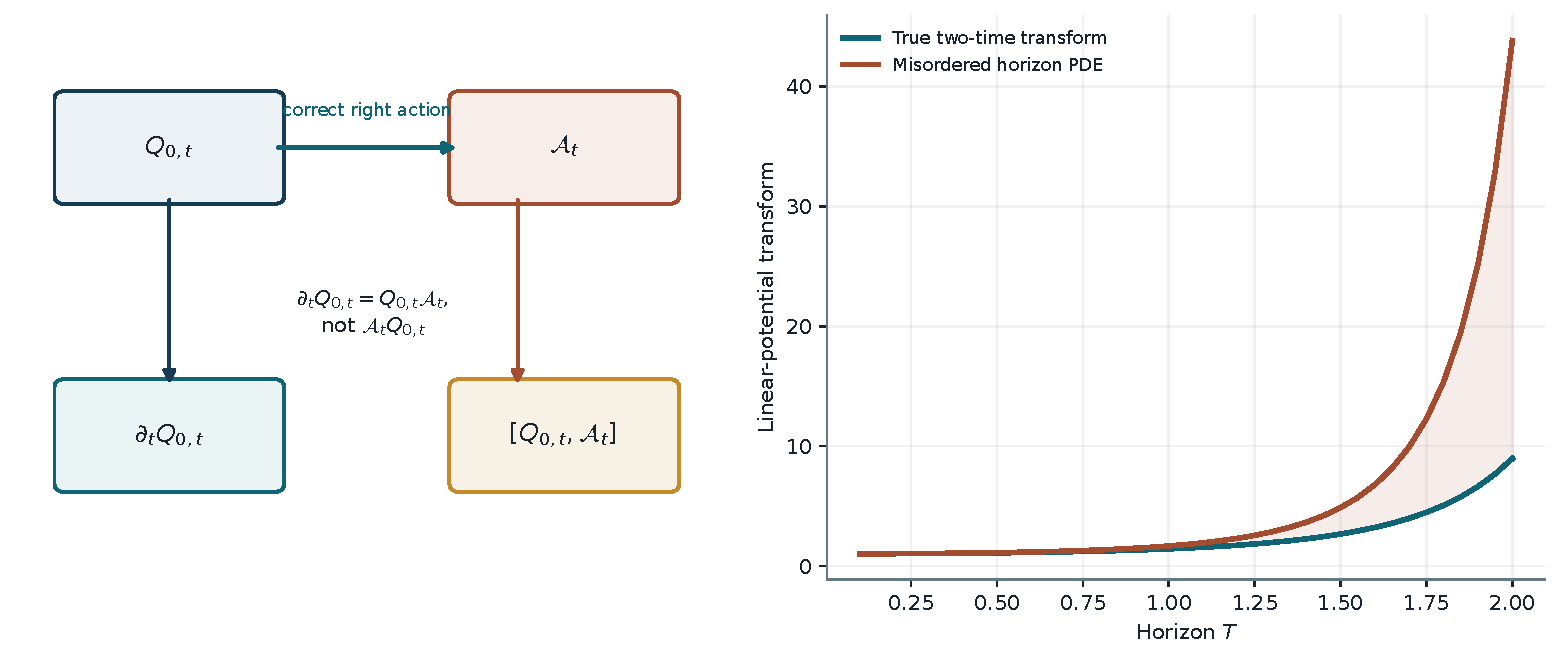
\includegraphics[width=1\linewidth,height=\textheight,keepaspectratio,alt={Two-panel figure. A diagram shows d Q over dt equals Q times A rather than A times Q; a plot shows the true transform and misordered PDE transform diverging rapidly with horizon.}]{figures/vector/f08_operator_ordering.pdf}

}

\caption{\label{fig-operator-order}Nonautonomous operator ordering. The
left panel distinguishes the correct right action from the invalid left
action; the right panel shows the resulting transform error in an
exactly solvable Gaussian example.}

\end{figure}%

\subsection{Maximal Gaussian scale symmetry}\label{sec-scale-symmetry}

Fix a horizon \([0,T_*]\). Let \(F:\mathbb R\to(-1,1)\) be a
homeomorphism and

\[
\rho_t=F(X_t/c),\qquad c>0,
\]

where

\begin{equation}\protect\phantomsection\label{eq-time-dependent-factor}{
X_t
=x_0+\int_0^t\mu(r)\,dr+\int_0^t\sigma(r)\,dW_r.
}\end{equation}

Assume deterministic \(x_0\), \(\mu\in L^1[0,T_*]\), and nonnegative
deterministic \(\sigma\in L^2[0,T_*]\). Equality of path laws means
equality as probability measures on \(C([0,T_*])\).

\begin{theorem}[Maximal Gaussian scale
equivalence]\protect\hypertarget{thm-scale-symmetry}{}\label{thm-scale-symmetry}

Two parameter sets produce the same path law for \(\rho\) if and only if

\begin{equation}\protect\phantomsection\label{eq-maximal-scale}{
\boxed{
\frac{x_0}{c}=\frac{x_0'}{c'},
\qquad
\frac{\mu(t)}{c}=\frac{\mu'(t)}{c'}
\quad\text{a.e.},
\qquad
\frac{\sigma(t)^2}{c^2}
=\frac{\sigma'(t)^2}{c'^2}
\quad\text{a.e.}
}
}\end{equation}

Under the nonnegative-volatility convention, the last equality is
equivalent to \(\sigma/c=\sigma'/c'\) almost everywhere.

\end{theorem}

\begin{proof}
Applying \(F^{-1}\) to the observed continuous path yields

\[
Y_t=\frac{X_t}{c}.
\]

This is a Gaussian process with mean

\[
m_Y(t)
=\frac{x_0}{c}
+\int_0^t\frac{\mu(r)}{c}\,dr
\]

and covariance

\[
C_Y(s,t)
=\int_0^{s\wedge t}
\frac{\sigma(r)^2}{c^2}\,dr.
\]

A Gaussian process law is determined by its mean and covariance.
Equality of the path laws therefore implies equality of the normalized
initial values and of the two integral functions. Absolute continuity
then gives the almost- everywhere coefficient equalities in
Eq.~\ref{eq-maximal-scale}. The converse follows by the same
mean/covariance characterization. \(\square\)
\end{proof}

For constant nonnegative coefficients, the positive scale orbit is

\begin{equation}\protect\phantomsection\label{eq-correct-scale-orbit}{
\boxed{
(x_0,c,\mu,\sigma)
\longmapsto
(\kappa x_0,\kappa c,\kappa\mu,\kappa\sigma),
\qquad \kappa>0.
}
}\end{equation}

Indeed, under the same Brownian path the normalized process is identical
pointwise. If signed diffusion coefficients are admitted, an additional
measurable sign gauge

\[
\sigma'(t)=\kappa\varepsilon(t)\sigma(t),
\qquad
\varepsilon(t)\in\{-1,1\},
\]

preserves the Gaussian law.

The previously written inverse action

\begin{equation}\protect\phantomsection\label{eq-incorrect-scale}{
(c,\mu,\sigma)
\mapsto
(\kappa c,\mu/\kappa,\sigma/\kappa)
}\end{equation}

is not an invariance. Starting with \(c=\sigma=1\) and \(\kappa=2\)
changes normalized volatility from \(1\) to \(1/4\), and normalized
variance at time \(t\) from \(t\) to \(t/16\).

This theorem is an identifiability statement, not an assertion that
scale can never be recovered. A direct observation of \(X\), an
externally fixed \(\sigma(t)\), or any dimensional measurement tied to
the latent coordinate breaks the orbit. One-dimensional scale
transformations and their hitting properties are classical (Itô and
McKean 1996).

\subsection{Joint endpoint--clock law}\label{sec-endpoint-clock}

Let

\[
A_t=\int_0^tf_c(X_s)\,ds
\]

for the constant-coefficient Gaussian factor Eq.~\ref{eq-factor}. Define
the tilted endpoint kernel

\begin{equation}\protect\phantomsection\label{eq-tilted-endpoint-kernel}{
K_\xi(t;x,y)\,dy
=E_x\left[
e^{i\xi A_t};X_t\in dy
\right].
}\end{equation}

It satisfies the forward equation

\begin{equation}\protect\phantomsection\label{eq-tilted-endpoint-pde}{
\boxed{
\partial_tK_\xi
=-\mu\partial_yK_\xi
+\frac{\nu^2}{2}\partial_{yy}K_\xi
+i\xi f_c(y)K_\xi,
\qquad
K_\xi(0;x,y)=\delta_x(y).
}
}\end{equation}

This is the standard additive-functional/Feynman--Kac construction (Kac
1949). Retaining \(y\) rather than integrating it out gives the joint
endpoint--clock transform without introducing a second spatial PDE
coordinate.

\begin{theorem}[Smooth endpoint--clock
density]\protect\hypertarget{thm-endpoint-clock}{}\label{thm-endpoint-clock}

Assume the joint diffusion is nonexplosive and its Stratonovich vector
fields are \(C^\infty\) with bounded derivatives of every order. For
every \(T>0\), \((A_T,X_T)\) has a smooth density. In the distributional
Fourier sense,

\begin{equation}\protect\phantomsection\label{eq-joint-density-inversion}{
\boxed{
p_{A_T,X_T}(a,y)
=\frac1{2\pi}
\int_{\mathbb R}
e^{-i\xi a}
K_\xi(T;x_0,y)\,d\xi.
}
}\end{equation}

Consequently,

\begin{equation}\protect\phantomsection\label{eq-clock-rho-density}{
\boxed{
p_{A_T,\rho_T}(a,r)
=\frac{c}{(1-r^2)^{3/2}}
p_{A_T,X_T}
\left(
a,\frac{cr}{\sqrt{1-r^2}}
\right).
}
}\end{equation}

\end{theorem}

\begin{proof}
In coordinates \((x,a)\), write the joint SDE in Stratonovich form.
Since the diffusion coefficient is constant, the Itô and Stratonovich
drifts coincide:

\[
V_1=\nu\partial_x,
\qquad
V_0=\mu\partial_x+f_c(x)\partial_a.
\]

Their bracket is

\[
[V_1,V_0]
=\nu f_c'(x)\partial_a.
\]

At every finite \(x\),

\[
f_c'(x)
=\frac{c^2}{(x^2+c^2)^{3/2}}>0.
\]

Thus \(V_1\) and \([V_1,V_0]\) span both tangent directions. The
parabolic, or weak, Hörmander condition holds, so the joint law has a
smooth density under the stated global hypotheses. Fourier
transformation in \(a\) gives Eq.~\ref{eq-tilted-endpoint-pde}, and
inverse Fourier transformation gives
Eq.~\ref{eq-joint-density-inversion}. The last formula is the monotone
Jacobian Eq.~\ref{eq-inverse}. \(\square\)
\end{proof}

The bracket argument belongs to classical hypoelliptic theory
(Kolmogoroff 1934; Hörmander 1967; Malliavin 1978; Kusuoka and Stroock
1985; Norris 1986; Nualart 2006; Hairer 2011; Delarue and Menozzi 2010).
It is not uniform: \(f_c'(x)\to0\) as \(|x|\to\infty\). The theorem
claims smoothness, not global Gaussian lower bounds or everywhere strict
positivity.

Pointwise use of Eq.~\ref{eq-joint-density-inversion} requires
additional Fourier decay, such as

\[
\xi\mapsto K_\xi(T;x_0,y)\in L^1(\mathbb R).
\]

Without it, distributional inversion is the correct statement.

For a corridor indicator

\[
O_T=\int_0^T\mathbf1_{\{\ell<X_s<h\}}\,ds,
\]

the geometry is different. The integrand is constant on open regions, so
paths can remain entirely outside or inside the corridor. Depending on
the initial point, the joint law may contain singular measures tied to
killed endpoint kernels: an atom at \(O_T=T\) is available when
\(x_0\in(\ell,h)\), while an atom at \(O_T=0\) is available when
\(x_0\notin[\ell,h]\). A boundary start can have neither because of
Brownian regularity. Any present singular components must be separated
before numerical inversion.

\subsection{Spectrally one-sided Lévy barriers}\label{sec-levy}

Let \(X\) be a spectrally negative Lévy process that is not the negative
of a subordinator. Write \(x=X_0\) and define its Laplace exponent by

\[
\psi(\theta)
=\log E[e^{\theta(X_1-X_0)}],
\qquad \theta\ge0.
\]

For \(\delta\ge0\), let \(\Phi(\delta)\) be the largest nonnegative
solution of

\[
\psi(\Phi(\delta))=\delta.
\]

Use the standard strict passage times

\begin{equation}\protect\phantomsection\label{eq-levy-passage-times}{
\tau_b^+
=\inf\{t>0:X_t>b\},
\qquad
\tau_a^-
=\inf\{t>0:X_t<a\}.
}\end{equation}

The \(\delta\)-scale function is zero on the negative half-line and is
normalized by

\[
W^{(\delta)}(x)=0,\quad x<0,
\]

\begin{equation}\protect\phantomsection\label{eq-scale-normalization}{
\boxed{
\int_0^\infty e^{-\theta y}W^{(\delta)}(y)\,dy
=\frac1{\psi(\theta)-\delta},
\qquad
\theta>\Phi(\delta).
}
}\end{equation}

Define

\begin{equation}\protect\phantomsection\label{eq-Z-scale}{
Z^{(\delta)}(x)
=1+\delta\int_0^xW^{(\delta)}(y)\,dy.
}\end{equation}

These conventions and the following identities are standard in
spectrally negative fluctuation theory (Bertoin 1996; Doney 2007;
Kyprianou 2014; Kuznetsov et al. 2013).

Let \(\rho_t=f_c(X_t)\) and \(r^*>\rho_0\). Set

\[
b=f_c^{-1}(r^*).
\]

Strict monotonicity gives the pathwise identity

\begin{equation}\protect\phantomsection\label{eq-monotone-barrier-transfer}{
\inf\{t>0:\rho_t>r^*\}
=\tau_b^+.
}\end{equation}

\begin{proposition}[One-sided bounded-factor fluctuation
identities]\protect\hypertarget{prp-levy-barriers}{}\label{prp-levy-barriers}

For \(x<b\),

\begin{equation}\protect\phantomsection\label{eq-upper-passage-transform}{
\boxed{
E_x[e^{-\delta\tau_b^+};\tau_b^+<\infty]
=e^{-\Phi(\delta)(b-x)}.
}
}\end{equation}

For \(a<x<b\),

\begin{equation}\protect\phantomsection\label{eq-two-sided-upper}{
\boxed{
E_x[e^{-\delta\tau_b^+};\tau_b^+<\tau_a^-]
=\frac{W^{(\delta)}(x-a)}
{W^{(\delta)}(b-a)},
}
}\end{equation}

and

\begin{equation}\protect\phantomsection\label{eq-two-sided-lower}{
\boxed{
E_x[e^{-\delta\tau_a^-};\tau_a^-<\tau_b^+]
=Z^{(\delta)}(x-a)
-Z^{(\delta)}(b-a)
\frac{W^{(\delta)}(x-a)}
{W^{(\delta)}(b-a)}.
}
}\end{equation}

\end{proposition}

\begin{proof}
The formulas for the driver are the standard one- and two-sided exit
identities. Equation Eq.~\ref{eq-monotone-barrier-transfer} transports
them pathwise to the bounded factor. No stochastic-calculus correction
appears because the argument concerns order of sample paths, not a
differential. \(\square\)
\end{proof}

The theory has a long development, including early resolvent
constructions, reflected exits, creeping, and scale-function regularity
(Suprun 1976; Avram et al. 2004; Alili and Kyprianou 2005; Chan et al.
2011). Occupation and joint occupation/first-passage transforms already
exist (Landriault et al. 2011; Loeffen et al. 2014), as does
state-dependent Omega killing (Li and Palmowski 2018).

Accordingly, Proposition~\ref{prp-levy-barriers} is a correction, not a
novelty theorem: reflection dies under jumps, but exact barriers do not
die universally. For two-sided VG or NIG drivers, this
one-scale-function simplification does not apply directly; Wiener--Hopf
or numerical fluctuation methods may remain available.

A sharper open problem begins from the existing generalized Omega-scale
Volterra equations and the bounded, sign-changing complex potential

\[
\omega_\xi(x)=\delta-i\xi f_c(x).
\]

The task is to prove the corresponding complex-valued two-sided exit and
resolvent identities rigorously, establish real-frequency decay or
\(L^1_\xi\) conditions, and construct a stable joint barrier--clock
inversion. Analytic continuation may be useful, but it is not itself the
required endpoint.

\section{Unified implications and limitations}\label{sec-implications}

\subsection{Exactness map}\label{exactness-map}

The paper's central distinction is between the failure of one
representation and the failure of tractability itself.

\begin{longtable}[]{@{}
  >{\raggedright\arraybackslash}p{(\linewidth - 12\tabcolsep) * \real{0.1429}}
  >{\raggedright\arraybackslash}p{(\linewidth - 12\tabcolsep) * \real{0.1429}}
  >{\raggedright\arraybackslash}p{(\linewidth - 12\tabcolsep) * \real{0.1429}}
  >{\raggedright\arraybackslash}p{(\linewidth - 12\tabcolsep) * \real{0.1429}}
  >{\raggedright\arraybackslash}p{(\linewidth - 12\tabcolsep) * \real{0.1429}}
  >{\raggedright\arraybackslash}p{(\linewidth - 12\tabcolsep) * \real{0.1429}}
  >{\raggedright\arraybackslash}p{(\linewidth - 12\tabcolsep) * \real{0.1429}}@{}}
\caption{Corrected exactness frontier. ``Exact'' includes a closed
transform or deterministic equation when no elementary density is
claimed.}\label{tbl-exactness-map}\tabularnewline
\toprule\noalign{}
\begin{minipage}[b]{\linewidth}\raggedright
Setting
\end{minipage} & \begin{minipage}[b]{\linewidth}\raggedright
Static law
\end{minipage} & \begin{minipage}[b]{\linewidth}\raggedright
Terminal European transform
\end{minipage} & \begin{minipage}[b]{\linewidth}\raggedright
Centered smile symmetry
\end{minipage} & \begin{minipage}[b]{\linewidth}\raggedright
Scalar terminal-clock barrier
\end{minipage} & \begin{minipage}[b]{\linewidth}\raggedright
Stationary observable law
\end{minipage} & \begin{minipage}[b]{\linewidth}\raggedright
Exact fixed-level factor barrier
\end{minipage} \\
\midrule\noalign{}
\endfirsthead
\toprule\noalign{}
\begin{minipage}[b]{\linewidth}\raggedright
Setting
\end{minipage} & \begin{minipage}[b]{\linewidth}\raggedright
Static law
\end{minipage} & \begin{minipage}[b]{\linewidth}\raggedright
Terminal European transform
\end{minipage} & \begin{minipage}[b]{\linewidth}\raggedright
Centered smile symmetry
\end{minipage} & \begin{minipage}[b]{\linewidth}\raggedright
Scalar terminal-clock barrier
\end{minipage} & \begin{minipage}[b]{\linewidth}\raggedright
Stationary observable law
\end{minipage} & \begin{minipage}[b]{\linewidth}\raggedright
Exact fixed-level factor barrier
\end{minipage} \\
\midrule\noalign{}
\endhead
\bottomrule\noalign{}
\endlastfoot
Independent Gaussian factor & exact pushforward & 1-D real-potential FK
& yes & yes for driftless linear combinations & no for scalar Brownian
state & reflection principle \\
Leveraged Gaussian factor & exact pushforward & 1-D complex FK &
generically no & not from \(J_T\) alone & no for scalar Brownian state &
reflection for the factor itself \\
Brownian Phase-Gram angles & exact Gaussian-angle pushforward &
finite-dimensional angle integral & not applicable & not applicable &
yes, compact pushforward & exact determinant-boundary survival \\
Nonautonomous Gaussian factor & exact finite-dimensional Gaussian law &
two-time backward or forward tilted PDE & under centered conditional law
& special time-change classes only & coefficient-dependent &
curved-boundary problem \\
Spectrally negative Lévy factor & exact transform pushforward & 1-D
PIDE/transform & driver-dependent & no Brownian reflection &
driver-dependent & fixed-level scale-function identities \\
Two-sided Lévy factor & exact transform pushforward & 1-D PIDE/transform
& driver-dependent & no & driver-dependent & no one-scale
simplification \\
\end{longtable}

\subsection{Correction ledger}\label{correction-ledger}

\begin{longtable}[]{@{}
  >{\raggedright\arraybackslash}p{(\linewidth - 2\tabcolsep) * \real{0.5000}}
  >{\raggedright\arraybackslash}p{(\linewidth - 2\tabcolsep) * \real{0.5000}}@{}}
\caption{Mathematical correction ledger for the bounded-factor
program.}\label{tbl-corrections}\tabularnewline
\toprule\noalign{}
\begin{minipage}[b]{\linewidth}\raggedright
Earlier statement
\end{minipage} & \begin{minipage}[b]{\linewidth}\raggedright
Correct statement
\end{minipage} \\
\midrule\noalign{}
\endfirsthead
\toprule\noalign{}
\begin{minipage}[b]{\linewidth}\raggedright
Earlier statement
\end{minipage} & \begin{minipage}[b]{\linewidth}\raggedright
Correct statement
\end{minipage} \\
\midrule\noalign{}
\endhead
\bottomrule\noalign{}
\endlastfoot
ATM implied correlation equals the mean clock. & It equals the mean
clock minus the exact square-root-variance Jensen term in
Eq.~\ref{eq-jensen-wedge}. \\
Leverage destroys conditional Gaussianity. & It introduces a random
conditional mean; Gaussianity and 1-D European transform closure
survive. \\
Brownian Phase-Gram has no stationary law. & Unwrapped angles have no
invariant law on \(\mathbb R^d\); matrix marginals converge to a compact
stationary pushforward. \\
The scale orbit uses inverse drift/volatility scaling. & All dimensional
latent parameters scale in the same direction as
Eq.~\ref{eq-correct-scale-orbit}. \\
Backward Feynman--Kac fails under calendar-time coefficients. & The
two-time theorem remains valid; a one-parameter left operator action is
misordered. \\
Lévy barriers are dead. & Brownian reflection is dead; one-sided
scale-function barriers remain exact. \\
\end{longtable}

\subsection{Limitations}\label{limitations}

\begin{enumerate}
\def\labelenumi{\arabic{enumi}.}
\tightlist
\item
  The implied-curvature theorem is local at the money. Global wings
  require the full mixture law.
\item
  The leveraged terminal transform is one-dimensional, but its potential
  is complex and strike inversion remains numerical.
\item
  The moving-boundary obstruction does not rule out exceptional
  leveraged barrier families.
\item
  The stationary Phase-Gram law is ordering-dependent,
  boundary-singular, and not LKJ for \(n\ge3\).
\item
  Stationarity of the matrix image does not prove a global Markov
  quotient generator at singular fibers.
\item
  Determinant asymptotics give only an upper bound on the smallest
  eigenvalue.
\item
  The endpoint--clock Hörmander condition is pointwise but not uniform.
\item
  Fourier inversion of the joint kernel is distributional unless
  frequency decay is established.
\item
  One-sided Lévy scale functions do not directly solve two-sided jump
  drivers.
\item
  The nonautonomous commutator formula requires a common invariant core
  and strong differentiability; unbounded-domain questions are real, not
  notation.
\end{enumerate}

\subsection{Open problems}\label{open-problems}

\begin{enumerate}
\def\labelenumi{\arabic{enumi}.}
\tightlist
\item
  \textbf{Leveraged barrier classification.} Characterize every nonzero
  leverage configuration for which the conditional calendar-time
  boundary is solvable, including strict clocks for which
  \(M_{J^{-1}(v)}\) is affine and degenerate clocks requiring no
  inverse.
\item
  \textbf{Higher smile derivatives.} Determine the complete ATM
  derivative hierarchy and which positive or negative moments of \(S\)
  it identifies.
\item
  \textbf{Mixture identifiability.} Decide when one full normal-implied
  smile uniquely determines the centered mixing distribution.
\item
  \textbf{Phase-Gram quotient dynamics.} Prove or disprove Markov
  lumpability of the matrix image, especially through boundary fibers.
\item
  \textbf{Spectral conditioning.} Derive sharp smallest-eigenvalue and
  condition- number asymptotics under \(\Pi_n\) and compare them with
  LKJ and Gram baselines.
\item
  \textbf{Leveraged endpoint--clock kernels.} Develop a stable joint
  transform for the endpoint and two additive functionals created by the
  Itô gauge.
\item
  \textbf{Complex Omega killing.} Starting from generalized Omega-scale
  Volterra equations, prove complex two-sided exit/resolvent identities
  for \(\delta-i\xi f_c(x)\), establish real-frequency decay, and
  construct a stable inversion.
\item
  \textbf{Observation channels and scale.} Classify which state-space
  observation schemes preserve or break Eq.~\ref{eq-maximal-scale}.
\end{enumerate}

\section{Conclusion}\label{sec-conclusion}

Bounded-factor tractability is not exhausted by independence, unwrapped
stationarity, time-homogeneous notation, or the Brownian reflection
principle. Each of those assumptions buys a particularly simple
representation. Removing one can destroy that representation without
destroying every exact structure.

For centered Gaussian variance mixtures, the ATM Bachelier level is
\(E[\sqrt V]\), not \(\sqrt{E[V]}\). In correlation units this
distinction is the exact Jensen wedge Eq.~\ref{eq-jensen-wedge}, and
clock dispersion pushes spread and basket implied correlations in
opposite directions. Under Brownian leverage, conditioning produces a
random mean and a residual clock. The explicit bounded-factor Itô gauge
and Fourier reduction preserve a one-dimensional European transform,
while the short-time third moment quantifies the resulting asymmetry.
For Brownian triangular angles, periodic quotienting produces a
stationary matrix law with exact determinant statistics and recurrent
boundary contact, even though the unwrapped angle lift diffuses forever.

The supporting corrections replace broad failure statements by precise
frontiers: simultaneous scale symmetry, two-time nonautonomous
evolution, hypoelliptic endpoint--clock smoothing, and one-sided Lévy
fluctuation identities.

The central closure principle is therefore

\[
\boxed{
\text{bounded factor}
+\text{Brownian leverage}
+\text{linear asset combination with terminal European payoff}
\Longrightarrow
\text{one-dimensional complex Feynman--Kac transform}.
}
\]

This principle is not universal: barriers retain the random mean path,
matrix stationarity is not automatically Markovianity, and two-sided
jumps exceed one-scale fluctuation theory. Its value is exactly that it
states what survives, what fails, and why.

\section{Technical appendices}\label{technical-appendices}

\subsection{Appendix A: Bachelier differentiation
ledger}\label{sec-app-bachelier}

Let \(d=k/s\). Starting from

\[
\mathcal B(s,k)=s\varphi(d)-k\Phi(-d),
\]

the derivatives used in Theorem~\ref{thm-mixture-smile} are:

\[
\partial_s[s\varphi(d)]
=\varphi(d)+s\varphi'(d)\left(-\frac{k}{s^2}\right)
=\varphi(d)+d^2\varphi(d),
\]

\[
\partial_s[-k\Phi(-d)]
=-k\varphi(d)\frac{k}{s^2}
=-d^2\varphi(d),
\]

so \(\mathcal B_s=\varphi(d)\). Likewise,

\[
\partial_k[s\varphi(d)]
=\varphi'(d)=-d\varphi(d),
\]

\[
\partial_k[-k\Phi(-d)]
=-\Phi(-d)+d\varphi(d),
\]

so \(\mathcal B_k=-\Phi(-d)\) and

\[
\mathcal B_{kk}=\frac{\varphi(d)}{s}.
\]

The remaining derivatives at \(k=0\) are

\[
\mathcal B_{sk}(s,0)=0,
\qquad
\mathcal B_{ss}(s,0)=0.
\]

These identities are sufficient for the implicit-function calculation;
no closed-form inversion away from ATM is used.

\subsection{Appendix B: Brownian covariance
algebra}\label{sec-app-leverage}

With the order \((W^1,W^2,W^0)\),

\[
\det\Sigma_W
=
\begin{vmatrix}
1&0&\ell_1\\
0&1&\ell_2\\
\ell_1&\ell_2&1
\end{vmatrix}
=1-\ell_1^2-\ell_2^2.
\]

Let the driver-loading matrix from \((W^1,W^2,W^0)\) to \((F_1,F_2,X)\)
be

\[
L(x)=
\begin{pmatrix}
\sigma_1&0&0\\
\sigma_2f_c(x)&\sigma_2s_c(x)&0\\
0&0&\nu
\end{pmatrix}.
\]

Then the covariance-rate matrix is

\[
\Sigma_{F,X}(x)=L(x)\Sigma_WL(x)^\top
\]

and

\[
\det\Sigma_{F,X}(x)
=(\det L(x))^2\det\Sigma_W
=\sigma_1^2\sigma_2^2\nu^2s_c(x)^2
(1-\ell_1^2-\ell_2^2).
\]

For the linear combination, \(g=(g_1,g_2)^\top\) and

\[
dZ_t=g(X_t)^\top
\left(
\ell\,dW_t^0+C\,dU_t
\right).
\]

Therefore

\[
h=\ell^\top g,\qquad
\Gamma=g^\top CC^\top g
=g^\top(I-\ell\ell^\top)g
=Q-h^2.
\]

\subsection{Appendix C: Generator expansion for
skewness}\label{sec-app-skew}

For a sufficiently regular test function \(\phi(x,y)\),

\[
\mathcal L\phi
=\mu\phi_x+\frac{\nu^2}{2}\phi_{xx}
+\frac{Q(x)}2\phi_{yy}
+\nu h(x)\phi_{xy}.
\]

Take \(\phi=y^3\). Then

\[
\phi_x=\phi_{xx}=\phi_{xy}=0,\qquad
\phi_{yy}=6y,
\]

so

\[
\mathcal L\phi=3yQ(x).
\]

For \(\psi(x,y)=3yQ(x)\),

\[
\psi_x=3yQ'(x),\quad
\psi_{xx}=3yQ''(x),\quad
\psi_{yy}=0,\quad
\psi_{xy}=3Q'(x).
\]

At \((x_0,0)\) only the mixed term survives:

\[
\mathcal L\psi(x_0,0)
=3\nu h(x_0)Q'(x_0).
\]

Under a local semigroup expansion,

\[
P_T\phi
=\phi+T\mathcal L\phi+\frac{T^2}{2}\mathcal L^2\phi+o(T^2),
\]

which proves Eq.~\ref{eq-third-moment}. Bounded \(Q\) supplies all
terminal moments; the expansion still requires the stated local
regularity.

\subsection{Appendix D: Phase-Gram Fourier and Beta
identities}\label{sec-app-phasegram}

Euler's formula gives

\[
\sin x=\frac{e^{ix}-e^{-ix}}{2i}.
\]

Raising to the even power \(2m\), pairing conjugate modes, and
collecting the zero mode yields Eq.~\ref{eq-sine-power-fourier}.
Gaussian-angle damping follows from

\[
E[e^{ik(\theta_0+\sigma W_t)}]
=e^{ik\theta_0-k^2\sigma^2t/2}.
\]

For \(U\) uniform on \([0,2\pi)\) and \(Y=\sin^2U\), the two preimages
in each half-period give

\[
f_Y(y)=\frac{1}{\pi\sqrt{y(1-y)}},
\qquad 0<y<1,
\]

the \(\operatorname{Beta}(1/2,1/2)\) density. Its logarithmic cumulant
generating function is

\[
\log E[Y^z]
=\log\Gamma(z+\tfrac12)-\log\Gamma(z+1)-\frac12\log\pi.
\]

Differentiation at zero gives the digamma and trigamma expressions used
in Eq.~\ref{eq-logdet-cumulants}.

\subsection{Appendix E: Killed-heat derivation of the singularity
time}\label{sec-app-exit}

For one angle shifted into \((0,\pi)\), the survival function solves

\[
\partial_tu=\frac{\sigma^2}{2}u_{xx},
\qquad
u(t,0)=u(t,\pi)=0,
\qquad
u(0,x)=1.
\]

Expand the constant initial condition in the Dirichlet sine basis:

\[
1
=\sum_{k=1}^\infty b_k\sin(kx),
\qquad
b_k=\frac2\pi\int_0^\pi\sin(kx)\,dx.
\]

Thus \(b_k=0\) for even \(k\) and

\[
b_{2m+1}=\frac4{\pi(2m+1)}.
\]

The heat semigroup multiplies the \(k\)th mode by
\(e^{-k^2\sigma^2t/2}\), producing Eq.~\ref{eq-angle-survival}.
Independence and the determinant product then give
Eq.~\ref{eq-singularity-survival}.

\subsection{Appendix F: Evolution-family commutator
derivation}\label{sec-app-commutator}

The derivation of Eq.~\ref{eq-commutator-defect} uses two different
strong derivatives:

\[
\partial_rQ_{0,r}=Q_{0,r}\mathcal A_r
\]

and

\[
\partial_rQ_{r,t}=-\mathcal A_rQ_{r,t}.
\]

They act on different sides because one changes the terminal time and
the other changes the initial time. This is the operator-level version
of the different weights \(r\) and \(T-r\) in the Gaussian diagnostic.
Domain invariance is indispensable when \(\mathcal A_t\) is unbounded.

\subsection{Appendix G: Gaussian path-law
identifiability}\label{sec-app-scale}

If two normalized Gaussian processes have the same law on
\(C([0,T_*])\), their finite-dimensional means and covariances agree.
Taking one time identifies the normalized mean function; taking pairs
identifies the integrated normalized variance. Conversely, equality of
those two functions gives equality of every finite-dimensional Gaussian
law. Continuity then identifies the path measure.

The theorem assumes a known common homeomorphism \(F\). If \(F\) itself
carries unknown scale or shape parameters, additional group actions can
appear and must be analyzed separately.

\subsection{Appendix H: Hypoelliptic and Lévy
conventions}\label{sec-app-hypo-levy}

The Hörmander bracket is computed for Stratonovich fields. Since the
sole diffusion field \(V_1=\nu\partial_x\) is constant, the
Itô-to-Stratonovich correction vanishes. The pointwise span is
two-dimensional, but the determinant of the spanning fields is
proportional to \(f_c'(x)\) and tends to zero at infinity.

For a spectrally negative Lévy process, \(W^{(\delta)}\) is continuous
on \([0,\infty)\) under the standing spectrally negative hypothesis, but
further differentiability depends on the Gaussian component and Lévy
measure (Chan et al. 2011). None of the exit formulas used in the main
text requires unqualified smoothness of the scale function.

Strict passage conventions match Kuznetsov et al. (2013). If non-strict
passage is desired, its equivalence must be checked against regularity
and creeping for the chosen process; the paper does not silently
interchange the two.

\subsection{Appendix I: Numerical evidence
ledger}\label{sec-app-numerics}

\begin{longtable}[]{@{}
  >{\raggedright\arraybackslash}p{(\linewidth - 2\tabcolsep) * \real{0.4286}}
  >{\raggedleft\arraybackslash}p{(\linewidth - 2\tabcolsep) * \real{0.5714}}@{}}
\caption{Selected deterministic and fixed-seed validation
anchors.}\label{tbl-numerical-ledger}\tabularnewline
\toprule\noalign{}
\begin{minipage}[b]{\linewidth}\raggedright
Check
\end{minipage} & \begin{minipage}[b]{\linewidth}\raggedleft
Value
\end{minipage} \\
\midrule\noalign{}
\endfirsthead
\toprule\noalign{}
\begin{minipage}[b]{\linewidth}\raggedright
Check
\end{minipage} & \begin{minipage}[b]{\linewidth}\raggedleft
Value
\end{minipage} \\
\midrule\noalign{}
\endhead
\bottomrule\noalign{}
\endlastfoot
Clock density mass & 1.000000000000 \\
\(E[A_T]\) & 0.106628721753 \\
\(\operatorname{Var}(A_T)\) & 0.111738386500 \\
Spread ATM implied correlation & 0.13453 \\
Basket ATM implied correlation & 0.08201 \\
Clock-density mean error versus independent quadrature &
\(-1.45\times10^{-6}\) \\
Clock-density variance error versus independent quadrature &
\(8.81\times10^{-7}\) \\
Maximum direct/conditional leveraged CF gap & 0.001627827791 \\
Maximum conditional/gauge CF gap & \(3.8689\times10^{-5}\) \\
Nonautonomous transform gap at \(T=1.3\) & 0.888672528169 \\
\end{longtable}

The evidence generator uses Python, NumPy, SciPy, and Matplotlib in the
existing project environment. It writes every plotted number to CSV or
JSON, uses seed 20260822, batches the leveraged simulation, and checks
Phase-Gram moments against independent terminal-angle simulation. The
exact formulas in the manuscript remain the canonical statements.

\section*{References}\label{references}
\addcontentsline{toc}{section}{References}

\protect\phantomsection\label{refs}
\begin{CSLReferences}{1}{1}
\bibitem[\citeproctext]{ref-acquistapaceterreni1987}
Acquistapace, Paolo, and Brunello Terreni. 1987. {``A Unified Approach
to Abstract Linear Nonautonomous Parabolic Equations.''}
\emph{Rendiconti Del Seminario Matematico Della Universit{à} Di Padova}
78: 47--107. \url{https://www.numdam.org/item/RSMUP_1987__78__47_0/}.

\bibitem[\citeproctext]{ref-alilikyprianou2005}
Alili, Larbi, and Andreas E. Kyprianou. 2005. {``Some Remarks on First
Passage of l{é}vy Processes, the American Put and Pasting Principles.''}
\emph{Annals of Applied Probability} 15 (3): 2062--80.
\url{https://doi.org/10.1214/105051605000000377}.

\bibitem[\citeproctext]{ref-alos2006}
Alòs, Elisa. 2006. {``A Generalization of the {Hull and White} Formula
with Applications to Option Pricing Approximation.''} \emph{Finance and
Stochastics} 10 (3): 353--65.
\url{https://doi.org/10.1007/s00780-006-0013-5}.

\bibitem[\citeproctext]{ref-alosbures2026}
Alòs, Elisa, and Òscar Burés Mogollón. 2026. {``Analytic Approximation
for {Bachelier} Option Prices and Applications.''} \emph{Entropy} 28
(6): 642. \url{https://doi.org/10.3390/e28060642}.

\bibitem[\citeproctext]{ref-alosgarcialorite2025}
Alòs, Elisa, and David García-Lorite. 2025. {``On the Curvature of the
{Bachelier} Implied Volatility.''} \emph{Risks} 13 (2): 27.
\url{https://doi.org/10.3390/risks13020027}.

\bibitem[\citeproctext]{ref-alosnualartpravosud2024}
Alòs, Elisa, Eulalia Nualart, and Makar Pravosud. 2024. {``On the
Implied Volatility of European and Asian Call Options Under the
Stochastic Volatility {Bachelier} Model.''} \emph{International Journal
of Theoretical and Applied Finance} 27 (7--8): 2550003.
\url{https://doi.org/10.1142/S0219024925500037}.

\bibitem[\citeproctext]{ref-andrewsmallows1974}
Andrews, David F., and Colin L. Mallows. 1974. {``Scale Mixtures of
Normal Distributions.''} \emph{Journal of the Royal Statistical Society:
Series B (Methodological)} 36 (1): 99--102.
\url{https://doi.org/10.1111/j.2517-6161.1974.tb00989.x}.

\bibitem[\citeproctext]{ref-applebaum2014}
Applebaum, David. 2014. \emph{Probability on Compact Lie Groups}. Vol.
70. Probability Theory and Stochastic Modelling. Springer.
\url{https://doi.org/10.1007/978-3-319-07842-7}.

\bibitem[\citeproctext]{ref-archakovhansenluo2024}
Archakov, Ilya, Peter Reinhard Hansen, and Yiyao Luo. 2024. {``A New
Method for Generating Random Correlation Matrices.''} \emph{The
Econometrics Journal} 27 (2): 188--212.
\url{https://doi.org/10.1093/ectj/utad027}.

\bibitem[\citeproctext]{ref-avramkyprianoupistorius2004}
Avram, Florin, Andreas E. Kyprianou, and Martijn R. Pistorius. 2004.
{``Exit Problems for Spectrally Negative l{é}vy Processes and
Applications to (Canadized) Russian Options.''} \emph{Annals of Applied
Probability} 14 (1): 215--38.
\url{https://doi.org/10.1214/aoap/1075828052}.

\bibitem[\citeproctext]{ref-bachelier1900}
Bachelier, Louis. 1900. {``Th{é}orie de La Sp{é}culation.''}
\emph{Annales Scientifiques de l'{É}cole Normale Sup{é}rieure}, 3rd
series, vol. 17: 21--86. \url{https://doi.org/10.24033/asens.476}.

\bibitem[\citeproctext]{ref-barnardmccullochmeng2000}
Barnard, John, Robert McCulloch, and Xiao-Li Meng. 2000. {``Modeling
Covariance Matrices in Terms of Standard Deviations and Correlations,
with Application to Shrinkage.''} \emph{Statistica Sinica} 10 (4):
1281--311. \url{https://www.jstor.org/stable/24306780}.

\bibitem[\citeproctext]{ref-barndorffnielsenkentsorensen1982}
Barndorff-Nielsen, Ole E., John T. Kent, and Michael Sørensen. 1982.
{``Normal Variance-Mean Mixtures and {\(z\)} Distributions.''}
\emph{International Statistical Review} 50 (2): 145--59.
\url{https://doi.org/10.2307/1402598}.

\bibitem[\citeproctext]{ref-bendelmickey1978}
Bendel, Robert B., and M. Ray Mickey. 1978. {``Population Correlation
Matrices for Sampling Experiments.''} \emph{Communications in
Statistics---Simulation and Computation} 7 (2): 163--82.
\url{https://doi.org/10.1080/03610917808812068}.

\bibitem[\citeproctext]{ref-bertoin1996}
Bertoin, Jean. 1996. \emph{L{é}vy Processes}. Vol. 121. Cambridge Tracts
in Mathematics. Cambridge University Press.

\bibitem[\citeproctext]{ref-blanescasasoteoros2009}
Blanes, Sergio, Fernando Casas, José A. Oteo, and José Ros. 2009. {``The
Magnus Expansion and Some of Its Applications.''} \emph{Physics Reports}
470 (5--6): 151--238.
\url{https://doi.org/10.1016/j.physrep.2008.11.001}.

\bibitem[\citeproctext]{ref-borodinsalminen2002}
Borodin, Andrei N., and Paavo Salminen. 2002. \emph{Handbook of Brownian
Motion---Facts and Formulae}. 2nd ed. Birkh{ä}user.
\url{https://doi.org/10.1007/978-3-0348-8163-0}.

\bibitem[\citeproctext]{ref-buccherietal2021}
Buccheri, Giuseppe, Giacomo Bormetti, Fulvio Corsi, and Fabrizio Lillo.
2021. {``A Score-Driven Conditional Correlation Model for Noisy and
Asynchronous Data: An Application to High-Frequency Covariance
Dynamics.''} \emph{Journal of Business \& Economic Statistics} 39 (4):
920--36. \url{https://doi.org/10.1080/07350015.2020.1739530}.

\bibitem[\citeproctext]{ref-carmonadurrleman2003}
Carmona, René A., and Valdo Durrleman. 2003. {``Pricing and Hedging
Spread Options.''} \emph{SIAM Review} 45 (4): 627--85.
\url{https://doi.org/10.1137/S0036144503424798}.

\bibitem[\citeproctext]{ref-chankyprianousavov2011}
Chan, Terence, Andreas E. Kyprianou, and Mladen Savov. 2011.
{``Smoothness of Scale Functions for Spectrally Negative l{é}vy
Processes.''} \emph{Probability Theory and Related Fields} 150 (3--4):
691--708. \url{https://doi.org/10.1007/s00440-010-0289-4}.

\bibitem[\citeproctext]{ref-choikimkwak2009}
Choi, Jaehyuk, Kwangmoon Kim, and Minsuk Kwak. 2009. {``Numerical
Approximation of the Implied Volatility Under Arithmetic Brownian
Motion.''} \emph{Applied Mathematical Finance} 16 (3): 261--68.
\url{https://doi.org/10.1080/13504860802583436}.

\bibitem[\citeproctext]{ref-choikwakteewang2022}
Choi, Jaehyuk, Minsuk Kwak, Chyng Wen Tee, and Yumeng Wang. 2022. {``A
{Black--Scholes} User's Guide to the {Bachelier} Model.''} \emph{Journal
of Futures Markets} 42 (5): 959--80.
\url{https://doi.org/10.1002/fut.22315}.

\bibitem[\citeproctext]{ref-clark1973}
Clark, Peter K. 1973. {``A Subordinated Stochastic Process Model with
Finite Variance for Speculative Prices.''} \emph{Econometrica} 41 (1):
135--55. \url{https://doi.org/10.2307/1913889}.

\bibitem[\citeproctext]{ref-daslangrene2022}
Das, Kaustav, and Nicolas Langrené. 2022. {``Closed-Form Approximations
with Respect to the Mixing Solution for Option Pricing Under Stochastic
Volatility.''} \emph{Stochastics} 94 (5): 745--88.
\url{https://doi.org/10.1080/17442508.2021.1993445}.

\bibitem[\citeproctext]{ref-delaruemenozzi2010}
Delarue, François, and Stéphane Menozzi. 2010. {``Density Estimates for
a Random Noise Propagating Through a Chain of Differential Equations.''}
\emph{Journal of Functional Analysis} 259 (6): 1577--630.
\url{https://doi.org/10.1016/j.jfa.2010.05.002}.

\bibitem[\citeproctext]{ref-doney2007}
Doney, Ronald A. 2007. \emph{Fluctuation Theory for l{é}vy Processes}.
Vol. 1897. Lecture Notes in Mathematics. Springer.
\url{https://doi.org/10.1007/978-3-540-48511-7}.

\bibitem[\citeproctext]{ref-driessenmaenhoutvilkov2009}
Driessen, Joost, Pascal J. Maenhout, and Grigory Vilkov. 2009. {``The
Price of Correlation Risk: Evidence from Equity Options.''} \emph{The
Journal of Finance} 64 (3): 1377--406.
\url{https://doi.org/10.1111/j.1540-6261.2009.01467.x}.

\bibitem[\citeproctext]{ref-duffiepansingleton2000}
Duffie, Darrell, Jun Pan, and Kenneth J. Singleton. 2000. {``Transform
Analysis and Asset Pricing for Affine Jump-Diffusions.''}
\emph{Econometrica} 68 (6): 1343--76.
\url{https://doi.org/10.1111/1468-0262.00164}.

\bibitem[\citeproctext]{ref-eastmanetal2016}
Eastman, Sean, Selwyn Hollis, Kawee Numpacharoen, and Jared Schlieper.
2016. {``The Volume of the Spatial Region Corresponding to
{\(n \times n\)} Correlation Matrices.''} \emph{The American
Mathematical Monthly} 123 (9): 909--18.
\url{https://doi.org/10.4169/amer.math.monthly.123.9.909}.

\bibitem[\citeproctext]{ref-escobargotzsecozagst2009}
Escobar, Marcos, Barbara Götz, Luis A. Seco, and Rudi Zagst. 2009.
{``Pricing of Spread Options on Stochastically Correlated
Underlyings.''} \emph{Journal of Computational Finance} 12 (3): 31--61.
\url{https://doi.org/10.21314/JCF.2009.205}.

\bibitem[\citeproctext]{ref-escobarkrausezagst2016}
Escobar, Marcos, Daniel Krause, and Rudi Zagst. 2016. {``Stochastic
Covariance and Dimension Reduction in the Pricing of Basket Options.''}
\emph{Review of Derivatives Research} 19 (3): 165--200.
\url{https://doi.org/10.1007/s11147-016-9119-x}.

\bibitem[\citeproctext]{ref-dafonsecagrassellitebaldi2007}
Fonseca, José da, Martino Grasselli, and Claudio Tebaldi. 2007.
{``Option Pricing When Correlations Are Stochastic: An Analytical
Framework.''} \emph{Review of Derivatives Research} 10 (2): 151--80.
\url{https://doi.org/10.1007/s11147-008-9018-x}.

\bibitem[\citeproctext]{ref-forresterzhang2020}
Forrester, Peter J., and Jiyuan Zhang. 2020. {``Parametrising
Correlation Matrices.''} \emph{Journal of Multivariate Analysis} 178:
104619. \url{https://doi.org/10.1016/j.jmva.2020.104619}.

\bibitem[\citeproctext]{ref-gourierouxsufana2010}
Gouriéroux, Christian, and Razvan Sufana. 2010. {``Derivative Pricing
with {Wishart} Multivariate Stochastic Volatility.''} \emph{Journal of
Business \& Economic Statistics} 28 (3): 438--51.
\url{https://doi.org/10.1198/jbes.2009.08105}.

\bibitem[\citeproctext]{ref-hairer2011}
Hairer, Martin. 2011. {``On Malliavin's Proof of h{ö}rmander's
Theorem.''} \emph{Bulletin Des Sciences Math{é}matiques} 135 (6--7):
650--66. \url{https://doi.org/10.1016/j.bulsci.2011.07.007}.

\bibitem[\citeproctext]{ref-haneanane2018}
Hanea, Anca M., and Gabriela F. Nane. 2018. {``The Asymptotic
Distribution of the Determinant of a Random Correlation Matrix.''}
\emph{Statistica Neerlandica} 72 (1): 14--33.
\url{https://doi.org/10.1111/stan.12113}.

\bibitem[\citeproctext]{ref-heston1993}
Heston, Steven L. 1993. {``A Closed-Form Solution for Options with
Stochastic Volatility with Applications to Bond and Currency Options.''}
\emph{Review of Financial Studies} 6 (2): 327--43.
\url{https://doi.org/10.1093/rfs/6.2.327}.

\bibitem[\citeproctext]{ref-holmes1991}
Holmes, R. B. 1991. {``On Random Correlation Matrices.''} \emph{SIAM
Journal on Matrix Analysis and Applications} 12 (2): 239--72.
\url{https://doi.org/10.1137/0612019}.

\bibitem[\citeproctext]{ref-hormander1967}
Hörmander, Lars. 1967. {``Hypoelliptic Second Order Differential
Equations.''} \emph{Acta Mathematica} 119: 147--71.
\url{https://doi.org/10.1007/BF02392081}.

\bibitem[\citeproctext]{ref-hullwhite1987}
Hull, John C., and Alan White. 1987. {``The Pricing of Options on Assets
with Stochastic Volatilities.''} \emph{The Journal of Finance} 42 (2):
281--300. \url{https://doi.org/10.1111/j.1540-6261.1987.tb02568.x}.

\bibitem[\citeproctext]{ref-itomckean1996}
Itô, Kiyosi, and Henry P. Jr. McKean. 1996. \emph{Diffusion Processes
and Their Sample Paths}. Classics in Mathematics. Springer.
\url{https://doi.org/10.1007/978-3-642-62025-6}.

\bibitem[\citeproctext]{ref-jaeckel2017}
Jäckel, Peter. 2017. {``Implied Normal Volatility.''} \emph{Wilmott}
2017 (88): 54--57. \url{https://doi.org/10.1002/wilm.10581}.

\bibitem[\citeproctext]{ref-joe2006}
Joe, Harry. 2006. {``Generating Random Correlation Matrices Based on
Partial Correlations.''} \emph{Journal of Multivariate Analysis} 97
(10): 2177--89. \url{https://doi.org/10.1016/j.jmva.2005.05.010}.

\bibitem[\citeproctext]{ref-johnsonkotzbalakrishnan1995}
Johnson, Norman L., Samuel Kotz, and N. Balakrishnan. 1995.
\emph{Continuous Univariate Distributions, Volume 2}. 2nd ed. John Wiley
\& Sons.

\bibitem[\citeproctext]{ref-kac1949}
Kac, Mark. 1949. {``On Distributions of Certain Wiener Functionals.''}
\emph{Transactions of the American Mathematical Society} 65 (1): 1--13.
\url{https://doi.org/10.1090/S0002-9947-1949-0027960-X}.

\bibitem[\citeproctext]{ref-karatzasshreve1991}
Karatzas, Ioannis, and Steven E. Shreve. 1991. \emph{Brownian Motion and
Stochastic Calculus}. 2nd ed. Vol. 113. Graduate Texts in Mathematics.
Springer. \url{https://doi.org/10.1007/978-1-4612-0949-2}.

\bibitem[\citeproctext]{ref-kato1953}
Kato, Tosio. 1953. {``Integration of the Equation of Evolution in a
Banach Space.''} \emph{Journal of the Mathematical Society of Japan} 5
(2): 208--34. \url{https://doi.org/10.2969/jmsj/00520208}.

\bibitem[\citeproctext]{ref-kolmogoroff1934}
Kolmogoroff, A. 1934. {``Zuf{ä}llige Bewegungen (Zur Theorie Der
Brownschen Bewegung).''} \emph{Annals of Mathematics} 35 (1): 116--17.
\url{https://doi.org/10.2307/1968123}.

\bibitem[\citeproctext]{ref-kusuokastroock1985}
Kusuoka, Shigeo, and Daniel W. Stroock. 1985. {``Applications of the
Malliavin Calculus. II.''} \emph{Journal of the Faculty of Science,
University of Tokyo, Section IA, Mathematics} 32 (1): 1--76.
\url{https://doi.org/10.15083/00039520}.

\bibitem[\citeproctext]{ref-kuznetsovkyprianourivero2013}
Kuznetsov, Alexey, Andreas E. Kyprianou, and Victor Rivero. 2013. {``The
Theory of Scale Functions for Spectrally Negative l{é}vy Processes.''}
In \emph{L{é}vy Matters II}, vol. 2061. Lecture Notes in Mathematics.
Springer. \url{https://doi.org/10.1007/978-3-642-31407-0_2}.

\bibitem[\citeproctext]{ref-kyprianou2014}
Kyprianou, Andreas E. 2014. \emph{Fluctuations of l{é}vy Processes with
Applications: Introductory Lectures}. 2nd ed. Springer.
\url{https://doi.org/10.1007/978-3-642-37632-0}.

\bibitem[\citeproctext]{ref-landriaultrenaudzhou2011}
Landriault, David, Jean-François Renaud, and Xiaowen Zhou. 2011.
{``Occupation Times of Spectrally Negative l{é}vy Processes with
Applications.''} \emph{Stochastic Processes and Their Applications} 121
(11): 2629--41. \url{https://doi.org/10.1016/j.spa.2011.07.008}.

\bibitem[\citeproctext]{ref-lewandowskikurowickajoe2009}
Lewandowski, Daniel, Dorota Kurowicka, and Harry Joe. 2009.
{``Generating Random Correlation Matrices Based on Vines and Extended
Onion Method.''} \emph{Journal of Multivariate Analysis} 100 (9):
1989--2001. \url{https://doi.org/10.1016/j.jmva.2009.04.008}.

\bibitem[\citeproctext]{ref-lipalmowski2018}
Li, Bo, and Zbigniew Palmowski. 2018. {``Fluctuations of Omega-Killed
Spectrally Negative l{é}vy Processes.''} \emph{Stochastic Processes and
Their Applications} 128 (10): 3273--99.
\url{https://doi.org/10.1016/j.spa.2017.10.018}.

\bibitem[\citeproctext]{ref-liao2004}
Liao, Ming. 2004. \emph{L{é}vy Processes in Lie Groups}. Vol. 162.
Cambridge Tracts in Mathematics. Cambridge University Press.
\url{https://doi.org/10.1017/CBO9780511546624}.

\bibitem[\citeproctext]{ref-lindersschoutens2014}
Linders, Daniël, and Wim Schoutens. 2014. {``A Framework for Robust
Measurement of Implied Correlation.''} \emph{Journal of Computational
and Applied Mathematics} 271: 39--52.
\url{https://doi.org/10.1016/j.cam.2014.03.026}.

\bibitem[\citeproctext]{ref-loeffenrenaudzhou2014}
Loeffen, Ronnie L., Jean-François Renaud, and Xiaowen Zhou. 2014.
{``Occupation Times of Intervals Until First Passage Times for
Spectrally Negative l{é}vy Processes.''} \emph{Stochastic Processes and
Their Applications} 124 (3): 1408--35.
\url{https://doi.org/10.1016/j.spa.2013.11.005}.

\bibitem[\citeproctext]{ref-lunardi1995}
Lunardi, Alessandra. 1995. \emph{Analytic Semigroups and Optimal
Regularity in Parabolic Problems}. Vol. 16. Progress in Nonlinear
Differential Equations and Their Applications. Birkh{ä}user.
\url{https://doi.org/10.1007/978-3-0348-9234-6}.

\bibitem[\citeproctext]{ref-ma2009}
Ma, Jun. 2009. {``A Stochastic Correlation Model with Mean Reversion for
Pricing Multi-Asset Options.''} \emph{Asia-Pacific Financial Markets} 16
(2): 97--109. \url{https://doi.org/10.1007/s10690-009-9088-2}.

\bibitem[\citeproctext]{ref-magnus1954}
Magnus, Wilhelm. 1954. {``On the Exponential Solution of Differential
Equations for a Linear Operator.''} \emph{Communications on Pure and
Applied Mathematics} 7 (4): 649--73.
\url{https://doi.org/10.1002/cpa.3160070404}.

\bibitem[\citeproctext]{ref-maher2012}
Maher, David G. 2012. {``Wrapping Brownian Motion and Heat Kernels. I:
Compact Lie Groups.''} \emph{Journal of Lie Theory} 22 (4): 1149--68.
\url{https://doi.org/10.5802/jolt.710}.

\bibitem[\citeproctext]{ref-malliavin1978}
Malliavin, Paul. 1978. {``Stochastic Calculus of Variations and
Hypoelliptic Operators.''} In \emph{Proceedings of the International
Symposium on Stochastic Differential Equations, Kyoto 1976}, edited by
Kiyosi Itô. Wiley.

\bibitem[\citeproctext]{ref-muirhead1982}
Muirhead, Robb J. 1982. \emph{Aspects of Multivariate Statistical
Theory}. John Wiley \& Sons.
\url{https://doi.org/10.1002/9780470316559}.

\bibitem[\citeproctext]{ref-norris1986}
Norris, James R. 1986. {``Simplified Malliavin Calculus.''} In
\emph{S{é}minaire de Probabilit{é}s XX}, vol. 1204. Lecture Notes in
Mathematics. Springer. \url{https://doi.org/10.1007/BFb0075716}.

\bibitem[\citeproctext]{ref-nualart2006}
Nualart, David. 2006. \emph{The Malliavin Calculus and Related Topics}.
2nd ed. Springer. \url{https://doi.org/10.1007/3-540-28329-3}.

\bibitem[\citeproctext]{ref-pazy1983}
Pazy, Amnon. 1983. \emph{Semigroups of Linear Operators and Applications
to Partial Differential Equations}. Vol. 44. Applied Mathematical
Sciences. Springer. \url{https://doi.org/10.1007/978-1-4612-5561-1}.

\bibitem[\citeproctext]{ref-pinheirobates1996}
Pinheiro, José C., and Douglas M. Bates. 1996. {``Unconstrained
Parametrizations for Variance-Covariance Matrices.''} \emph{Statistics
and Computing} 6 (3): 289--96. \url{https://doi.org/10.1007/BF00140873}.

\bibitem[\citeproctext]{ref-poitras1998}
Poitras, Geoffrey. 1998. {``Spread Options, Exchange Options, and
Arithmetic Brownian Motion.''} \emph{Journal of Futures Markets} 18 (5):
487--517.
\url{https://doi.org/10.1002/(SICI)1096-9934(199808)18:5\%3C487::AID-FUT1\%3E3.0.CO;2-Z}.

\bibitem[\citeproctext]{ref-pourahmadiwang2015}
Pourahmadi, Mohsen, and Xiao Wang. 2015. {``Distribution of Random
Correlation Matrices: Hyperspherical Parameterization of the Cholesky
Factor.''} \emph{Statistics \& Probability Letters} 106: 5--12.
\url{https://doi.org/10.1016/j.spl.2015.06.015}.

\bibitem[\citeproctext]{ref-rapisardabrigomercurio2007}
Rapisarda, Francesco, Damiano Brigo, and Fabio Mercurio. 2007.
{``Parameterizing Correlations: A Geometric Interpretation.''} \emph{IMA
Journal of Management Mathematics} 18 (1): 55--73.
\url{https://doi.org/10.1093/imaman/dpl010}.

\bibitem[\citeproctext]{ref-rebonatojackel2000}
Rebonato, Riccardo, and Peter Jäckel. 2000. {``The Most General
Methodology for Creating a Valid Correlation Matrix for Risk Management
and Option Pricing Purposes.''} \emph{The Journal of Risk} 2 (2):
17--27. \url{https://doi.org/10.21314/JOR.2000.023}.

\bibitem[\citeproctext]{ref-renaulttouzi1996}
Renault, Éric, and Nizar Touzi. 1996. {``Option Hedging and Implied
Volatilities in a Stochastic Volatility Model.''} \emph{Mathematical
Finance} 6 (3): 279--302.
\url{https://doi.org/10.1111/j.1467-9965.1996.tb00117.x}.

\bibitem[\citeproctext]{ref-rolloos2022}
Rolloos, Frido. 2022. \emph{{Hull and White} and {Al{ò}s} Type Formulas
for Barrier Options in Stochastic Volatility Models with Nonzero
Correlation}. \url{https://doi.org/10.48550/arXiv.2205.05489}.

\bibitem[\citeproctext]{ref-romanotouzi1997}
Romano, Marc, and Nizar Touzi. 1997. {``Contingent Claims and Market
Completeness in a Stochastic Volatility Model.''} \emph{Mathematical
Finance} 7 (4): 399--412. \url{https://doi.org/10.1111/1467-9965.00038}.

\bibitem[\citeproctext]{ref-rouault2007}
Rouault, Alain. 2007. {``Asymptotic Behavior of Random Determinants in
the Laguerre, Gram and Jacobi Ensembles.''} \emph{ALEA---Latin American
Journal of Probability and Mathematical Statistics} 3: 181--230.
\url{https://arxiv.org/abs/math/0607767}.

\bibitem[\citeproctext]{ref-scott1997}
Scott, Louis O. 1997. {``Pricing Stock Options in a Jump-Diffusion Model
with Stochastic Volatility and Interest Rates: Applications of Fourier
Inversion Methods.''} \emph{Mathematical Finance} 7 (4): 413--26.
\url{https://doi.org/10.1111/1467-9965.00039}.

\bibitem[\citeproctext]{ref-skintzirefenes2005}
Skintzi, Vasiliki D., and Apostolos-P. N. Refenes. 2005. {``Implied
Correlation Index: A New Measure of Diversification.''} \emph{Journal of
Futures Markets} 25 (2): 171--97.
\url{https://doi.org/10.1002/fut.20137}.

\bibitem[\citeproctext]{ref-springerthompson1970}
Springer, M. D., and W. E. Thompson. 1970. {``The Distribution of
Products of Beta, Gamma and Gaussian Random Variables.''} \emph{SIAM
Journal on Applied Mathematics} 18 (4): 721--37.
\url{https://doi.org/10.1137/0118065}.

\bibitem[\citeproctext]{ref-suprun1976}
Suprun, V. N. 1976. {``Problem of Destruction and Resolvent of a
Terminating Process with Independent Increments.''} \emph{Ukrainian
Mathematical Journal} 28 (1): 39--45.
\url{https://doi.org/10.1007/BF01559226}.

\bibitem[\citeproctext]{ref-tanggupta1984}
Tang, Jen, and A. K. Gupta. 1984. {``On the Distribution of the Product
of Independent Beta Random Variables.''} \emph{Statistics \& Probability
Letters} 2 (3): 165--68.
\url{https://doi.org/10.1016/0167-7152(84)90008-7}.

\bibitem[\citeproctext]{ref-willard1997}
Willard, Gregory A. 1997. {``Calculating Prices and Sensitivities for
Path-Independent Derivative Securities in Multifactor Models.''}
\emph{Journal of Derivatives} 5 (1): 45--61.
\url{https://doi.org/10.3905/jod.1997.407982}.

\end{CSLReferences}




\end{document}
